\begin{beginSngnote}
    Si tenga presente che alcuni termini utilizzati nel documento riportano la lettera \textbf{G} in apice, allo scopo di evidenziare le parole che assumono uno specifico significato nell'ambito del progetto. Per comprenderle in maniera corretta, si rimanda il lettore al documento ``Glossario", che contiene un elenco completo di tutte le terminologie utilizzate con relative definizioni, allo scopo di costruire un linguaggio uniforme che possa migliorare la comunicazione tra i componenti interni al gruppo e gli stakeholders\textsuperscript{G} esterni.   %inserire corsivo per ogni termine del glossario?
\end{beginSngnote}

%unire scopo delcoumento e il progetto in un unica sezione  (e.g. introduzione) con due sottosezioni?
%%%%%%%%%%%%%%%%%%%%%%%%%%%%%%%%%%%
% SCOPO DEL DOCUMENTO
%%%%%%%%%%%%%%%%%%%%%%%%%%%%%%%%%%%

\section{Introduzione}

\subsection{Scopo del documento}\label{sec:scopo_del_documento}
\par Questo documento definisce come le attività di controllo della qualità saranno gestite durante il ciclo di vita del prodotto software. Include dettagli sui processi e standard da seguire per assicurare che il prodotto finale rispetti i requisiti di qualità specificati. Questo piano è fondamentale per garantire che il software sviluppato sia di alta qualità e soddisfi le aspettative dei clienti e degli stakeholder. Al suo interno contiene le metriche per misurare il livello di qualità di progetto in fase di sviluppo, in modo da poter migliorare alcune procedure se giudicate non conformi alle aspettative. Si prevede che il documento abbia natura incrementale, perché le metriche potrebbero essere aggiornate o riadattate in corso di progetto, a seconda delle esigenze e delle richieste da parte del committente.
\par Nel corso di progetto, l'accertamento della qualità sarà documentato allegando al documento le misurazioni delle attività di verifica con le metriche descritte.

%%%%%%%%%%%%%%%%%%%%%%%%%%%%%%%%%%%
% IL PROGETTO
%%%%%%%%%%%%%%%%%%%%%%%%%%%%%%%%%%%
\subsection{Il progetto}\label{sec:il_progetto}
\par Il progetto nasce nell'ambito dei \textbf{sistemi gestionali di magazzino}, meglio noti con il termine inglese di \textit{Warehouse Management Systems} (WMS), con l'obiettivo di risolvere una serie di problematiche derivanti dalle soluzioni tradizionali tuttora presenti sul mercato.
\par Il focus principale sarà migliorare la user experience, tramite la realizzazione di un applicativo che proponga all'utente un'interazione con il magazzino in un ambiente di lavoro 3D: questa soluzione, rispetto ai tradizionali sistemi 2D, garantirebbe una maggiore comprensione degli spazi, proponendo una visualizzazione più intuitiva e familiare del magazzino all'utente che, di conseguenza, sarà in grado di prendere decisioni organizzative più informate ed efficienti, ottimizzando i processi di logistica.
\par Per raggiungere questo obiettivo, l'ambiente di lavoro non può essere una semplice visualizzazione del magazzino. L'utente dovrà infatti poter:
\begin{itemize}
    \item Navigare l'ambiente 3D;
    \item Progettare la scaffalatura e modificarla nel tempo;
    \item Inserire, spostare e rimuovere prodotti negli scaffali.
\end{itemize}
Il progetto deve concretizzarsi nella realizzazione di una web app fruibile agli impiegati d'ufficio ed incentrata sulla visualizzazione 3D del magazzino.
\par Per visionare il capitolato\textsuperscript{G} e la documentazione del gruppo, si veda la sezione \hyperref[sec:riferimenti_esterni]{Riferimenti Esterni} del documento.

\newpage

%%%%%%%%%%%%%%%%%%%%%%%%%%%%%%%%%%%
% QUALITA' DI PROCESSO
%%%%%%%%%%%%%%%%%%%%%%%%%%%%%%%%%%%
\section{Obiettivi metrici di qualità}\label{sec:obiettivi_metrici}
In questa sezione si presentano i valori accettabili e ideali delle metriche, insieme ad una breve descrizione delle stesse. Le metriche descritte nel documento saranno identificate univocamente tramite un codice standardizzato secondo quanto definito nelle \textit{Norme di Progetto}, reperibili nella sezione \hyperref[sec:riferimenti_esterni]{Riferimenti Esterni} del documento.

\subsection{Qualità di processo}\label{sec:qualita_di_processo}
Questa sezione è dedicata alle metriche atte a misurare la qualità dei processi nel corso del progetto didattico, qui descritti seguendo lo standard \textbf{ISO/IEC 12207}, reperibile nella sezione \hyperref[sec:riferimenti_esterni]{Riferimenti Esterni} del documento. 
\subsubsection{Processi primari}
\paragraph{Fornitura}
Uno dei compiti principali del processo di fornitura è la gestione delle procedure e delle risorse necessarie a garantire il raggiungimento degli obiettivi di progetto. Per questo motivo, le metriche di qualità adottate in questo processo hanno lo scopo di misurare come il progetto si sta muovendo rispetto alla sua pianificazione originaria, in termini di costi previsti in partenza rispetto ai costi effettivi nel corso di progetto.
\par Risulta subito evidente il fatto che delle semplici metriche di monitoraggio dei tempi non sono abbastanza per comprendere lo stato effettivo del progetto (molte ore di lavoro non significano sempre che il prodotto da realizzare è a buon punto) e per questo non possono garantire un buon livello di qualità. Per questo motivo, il gruppo ha scelto di utilizzare le metriche proposte dal metodo \textbf{Earned Value}, che si propone di misurare la quantità di lavoro effettivamente eseguito su un progetto.
\par Gli acronimi utilizzati nelle metriche faranno riferimento a quelli proposti dallo standard, reperibili al link sulle metriche di progetto nella sezione \hyperref[sec:riferimenti_esterni]{Riferimenti Esterni}. Per una lettura più immediata del documento si riportano i termini principali:
\begin{table}[h!]
\centering
\def\arraystretch{1.5}
\begin{tabular}{ |m{2cm}|m{4cm}|m{8cm}| }
\hline
\rowcolor{lightgray!30}
\textbf{Acronimo} & \textbf{Nome} & \textbf{Significato}\\
\hline
\textbf{PV} & Planned Value & Costo pianificato per realizzare le attività di progetto alla data corrente.\\
\hline
\textbf{AC} & Actual Cost & Costo effettivamente sostenuto alla data corrente.\\
\hline
\textbf{EV} & Earned Value & Valore delle attività realizzate alla data corrente.\\
\hline
\textbf{BAC} & Budget at Completion & Indica il valore iniziale previsto per la realizzazione del progetto.\\
\hline
\textbf{ETC} & Estimate to Complete & Valore stimato per la realizzazione delle rimanenti attività necessarie al completamento del progetto.\\
\hline
\textbf{EAC} & Estimated at Completion & Indica la revisione del BAC rispetto allo stato corrente del progetto (EAC = AC + ETC).\\
\hline
\textbf{CV} & Cost Variance & Calcola il valore del costo realmente maturato rispetto al costo effettivo (CV = EV - AC).\\
\hline
\textbf{SV} & Schedule Variance & Calcola le tempistiche effettive (se si è in anticipo o ritardo) rispetto alla schedulazione delle attività pianificate (SV = EV - PV).\\
\hline
\textbf{BV} & Budget Variance & Indica se alla data corrente si è speso di più o di meno rispetto a quanto previsto (BV = PV - AC).\\
\hline
\end{tabular}
\end{table}

\newpage
Le metriche sono stabilite di conseguenza:
\begin{table}[h!]
\rowcolors{2}{lightgray!30}{white}
\centering
\def\arraystretch{1.5}
\begin{tabular}{ |>{\centering\arraybackslash}m{2.5cm}|>{\centering\arraybackslash}m{5.5cm}|>{\centering\arraybackslash}m{3cm}|>{\centering\arraybackslash}m{3cm}| }
\hline
\rowcolor{black}
\textbf{\color{white} Codice} & \textbf{\color{white} Descrizione} & \textbf{\color{white} Valore accettabile} & \textbf{\color{white} Valore ottimale}\\
\hline
MPC1-EAC & Si vuole che il costo attuale sia quanto più possibile in linea con quello pianificato originariamente & Errore massimo del $\pm 5$\% rispetto a BAC & = BAC \\
\hline
MPC2-CV & Si vuole che il valore delle attività completate (EV) sia corrispondente o maggiore del costo sostenuto (AC) & $\geq$ -10\% & $\geq$ 0 \\
\hline
MPC3-SV & Si vuole che il progetto produca con maggiore o uguale velocità rispetto a quanto pianificato & $\geq$ -10\% & $\geq$ 0 \\
\hline
MPC4-BV & Si vuole che i costi previsti nella pianificazione iniziale corrispondano a quelli effettivi & Errore massimo del $\pm 10$\% & 0 \\
\hline
MPC5-PV & I costi pianificati per le attività di progetto non devono sforare i costi originariamente pianificati & - & La somma dei costi di volta in volta deve essere $\leq$ BAC \\
\hline
MPC6-AC & I costi effettivi per le attività di progetto non devono sforare i costi pianificati nella revisione del BAC & - & La somma dei costi di volta in volta deve essere $\leq$ EAC \\
\hline
MPC7-EV & Il valore effettivo per le attività di progetto non deve sforare i costi pianificati nella revisione del BAC & - & La somma dei costi di volta in volta deve essere $\leq$ EAC \\
\hline
\end{tabular}
\end{table}

\paragraph{Sviluppo}
Il processo di sviluppo definisce i compiti e le attività che il gruppo deve svolgere per la
realizzazione del prodotto software concorde con le esigenze del proponente ed, in particolare, si occupa delle attività di analisi dei requisiti, progettazione e codifica. Le metriche di qualità individuate per questo processo sono relative soprattutto alle ultime due attività.
\subparagraph{Progettazione.} Per assicurare qualità nella fase di progettazione si è ritenuto importante utilizzare le metriche di \textbf{Structural fan-in} e \textbf{fan-out}, applicate alle procedure con i seguenti acronimi:
\begin{table}[h!]
\centering
\def\arraystretch{1.5}
\begin{tabular}{ |m{2cm}|m{4cm}|m{8cm}| }
\hline
\rowcolor{lightgray!30}
\textbf{Acronimo} & \textbf{Nome} & \textbf{Signficato}\\
\hline
\textbf{SFINp} & Structural fan-in (procedure) & Numero di procedure che chiamano una specifica procedura.\\
\hline
\textbf{SFOUTp} & Structural fan-out (procedure) & Numero di procedure che una specifica procedura chiama.\\
\hline
\end{tabular}
\end{table}

\newpage
Le regole da applicare alle metriche sono dunque le seguenti:
\begin{table}[h!]
\rowcolors{2}{lightgray!30}{white}
\centering
\def\arraystretch{1.5}
\begin{tabular}{ |>{\centering\arraybackslash}m{4cm}|>{\centering\arraybackslash}m{5.5cm}|>{\centering\arraybackslash}m{5cm}| }
\hline
\rowcolor{black}
\textbf{\color{white} Codice} & \textbf{\color{white} Descrizione} & \textbf{\color{white} Valore desiderabile}\\
\hline
MPC8-SFINp & Si vuole che le procedure progettate vengano riutilizzate & Alto (riutilizzo di codice) \\
\hline
MPC9-SFOUTp & Si vuole che le procedure non siano fortemente accoppiate fra loro & Basso (bassa dipendenza tra procedure) \\
\hline
\end{tabular}
\end{table}


\subparagraph{Codifica.}
Con l'attività di codifica, i programmatori si impegnano a concretizzare quanto prodotto con l'attività di progettazione attraverso la programmazione del software vero e proprio.
Lo scopo è quello di ottenere un prodotto software che rispetti i requisti e le richieste concordati con il proponente e che ne garantisca la qualità. Per raggiungere questi obiettivi si utilizzano metriche che cercano di limitare gli errori introdotti nel codice, in particolare:
\begin{table}[h!]
\centering
\def\arraystretch{1.5}
\begin{tabular}{ |m{2cm}|m{2.5cm}|m{9.5cm}| }
\hline
\rowcolor{lightgray!30}
\textbf{acronimo} & \textbf{Nome} & \textbf{signficato}\\
\hline
\textbf{CCH} & Code churn & Indica il numero di modifiche, aggiunte e cancellazioni apportate nel tempo ad una certa area di codice, in particolare nell'ambito di progetto, si intende modifiche apportate ad una procedura. Più sono le modifiche, più aumenta il rischio di introdurre errori nel codice. Un alto valore di nuove linee di codice potrebbe anche indicare basso riutilizzo di codice.\\
\hline
\textbf{NB} & Number of bugs & Indica il numero di bug ed errori presenti nel software.\\
\hline
\textbf{CC} & Cyclomatic complexity & Misura la complessità del codice calcolando il numero di percorsi indipendenti (contando cioè il numero di ``decisioni prese" nel codice sorgente). Un alto valore di complessità ciclomatica\textsuperscript{G} indica codice difficile da comprendere, mantenere e testare.\\
\hline
\end{tabular}
\end{table}
\par Le regole di qualità sono applicate alle metriche nel seguente modo:
\begin{table}[h!]
\rowcolors{2}{lightgray!30}{white}
\centering
\def\arraystretch{1.5}
\begin{tabular}{ |>{\centering\arraybackslash}m{2.5cm}|>{\centering\arraybackslash}m{5.5cm}|>{\centering\arraybackslash}m{3cm}|>{\centering\arraybackslash}m{3cm}| }
\hline
\rowcolor{black}
\textbf{\color{white} Codice} & \textbf{\color{white} Descrizione} & \textbf{\color{white} Valore accettabile} & \textbf{\color{white} Valore ottimale}\\
\hline
MPC10-CCH & Il numero di modifiche apportate alla singola procedura deve essere quanto più basso possibile & massimo 20\% di modifiche sul codice totale della procedura & 0 \\
\hline
MPC11-NB & Si vuole che il numero di bug ed errori nel codice sia quanto più basso possibile & $\leq$ 5 & 0 \\
\hline
MPC12-CC & Il codice deve essere mantenuto semplice, facilitando comprensione, manutenzione e test & $\leq$ 15 & $\leq$ 10 \\
\hline
\end{tabular}
\end{table}

\subsubsection{Processi di supporto}
\paragraph{Documentazione}
La documentazione prodotta nel corso del progetto deve essere un valido supporto al gruppo e agli stakeholders per comprendere meglio il codice prodotto, le decisioni prese e la gestione orgaSzzativa. Per questo motivo, le metriche di qualità sulla documentazione si concentrano sulla leggibilità e sul controllo degli errori ortografici. Le metriche in questione sono le seguenti:
\begin{table}[h!]
\centering
\def\arraystretch{1.5}
\begin{tabular}{ |m{2cm}|m{4.5cm}|m{7.5cm}| }
\hline
\rowcolor{lightgray!30}
\textbf{acronimo} & \textbf{Nome} & \textbf{signficato}\\
\hline
\textbf{EOD} & Errori ortografici per documento & Indica il numero di errori ortografici individuati per documento.\\
\hline
\textbf{IG} & Indice Gulpease & Calcola la leggibilità di un testo in lingua italiana prendendo in considerazione la lunghezza della parola e la lunghezza della frase rispetto al numero di lettere. 
\begin{center}
    $89 + \ddfrac{300 * (num.\: frasi) - 10 * (num.\: lettere)}{(num.\: parole)} $
\end{center}\\
\hline
\end{tabular}
\end{table}
\par Le regole di qualità sono applicate alle metriche nel seguente modo:
\begin{table}[h!]
\rowcolors{2}{lightgray!30}{white}
\centering
\def\arraystretch{1.5}
\begin{tabular}{ |>{\centering\arraybackslash}m{2.5cm}|>{\centering\arraybackslash}m{5.5cm}|>{\centering\arraybackslash}m{3cm}|>{\centering\arraybackslash}m{3cm}| }
\hline
\rowcolor{black}
\textbf{\color{white} Codice} & \textbf{\color{white} Descrizione} & \textbf{\color{white} Valore accettabile} & \textbf{\color{white} Valore ottimale}\\
\hline
MPC13-EOD & Si vogliono meno errori ortografici possibili per ciascun documento & $\leq 5$ & 0 \\
\hline
MPC14-IG & La documentazione deve essere di facile lettura & 30-100 & 40-100 \\
\hline
\end{tabular}
\end{table}

\paragraph{Accertamento della qualità}
Lo scopo dell'accertamento della qualità è garantire che i processi e il prodotto siano conformi alle attese e soddisfino al meglio le richieste del proponente. A tal fine e per avere una valutazione oggettiva e quantificabile della qualità, si fa riferimento al presente \textit{Piano di Qualifica}, che riporta le metriche di qualità adottate dal gruppo nell'ambito del progetto.
\par Diventa quindi essenziale il soddisfacimento delle metriche preposte:
\begin{table}[h!]
\centering
\def\arraystretch{1.5}
\begin{tabular}{ |m{2cm}|m{3.5cm}|m{8.5cm}| }
\hline
\rowcolor{lightgray!30}
\textbf{acronimo} & \textbf{Nome} & \textbf{signficato}\\
\hline
\textbf{MS} & Metriche soddisfatte & Indica la percentuale di metriche di qualità soddisfatte rispetto al totale delle metriche preposte.\\
\hline
\end{tabular}
\end{table}
\par Con le seguenti regole:
\begin{table}[h!]
\rowcolors{2}{lightgray!30}{white}
\centering
\def\arraystretch{1.5}
\begin{tabular}{ |>{\centering\arraybackslash}m{2.5cm}|>{\centering\arraybackslash}m{5.5cm}|>{\centering\arraybackslash}m{3cm}|>{\centering\arraybackslash}m{3cm}| }
\hline
\rowcolor{black}
\textbf{\color{white} Codice} & \textbf{\color{white} Descrizione} & \textbf{\color{white} Valore accettabile} & \textbf{\color{white} Valore ottimale}\\
\hline
MPC15-MS & Il numero di metriche di qualità soddisfatte deve essere molto alto & 90\% & 100\% \\
\hline
\end{tabular}
\end{table}

\newpage
\paragraph{Verifica}
Il processo di verifica ha lo scopo di determinare se i prodotti dei processi durante il corso del progetto rispettano i requisiti preposti. In particolare, si vuole enfatizzare la correttezza del codice prodotto attraverso le seguenti metriche:
\begin{table}[h!]
\centering
\def\arraystretch{1.5}
\begin{tabular}{ |m{2cm}|m{3.5cm}|m{8.5cm}| }
\hline
\rowcolor{lightgray!30}
\textbf{acronimo} & \textbf{Nome} & \textbf{signficato}\\
\hline
\textbf{CCV} & Code coverage & Misura la quantità di codice (in percentuale) coperta dai test rispetto al totale del codice sorgente.\\
\hline
\textbf{TP} & Test passati & Misura la quantità di test (in percentuale) eseguiti con successo.\\
\hline
\end{tabular}
\end{table}
\par Con le seguenti regole:
\begin{table}[h!]
\rowcolors{2}{lightgray!30}{white}
\centering
\def\arraystretch{1.5}
\begin{tabular}{ |>{\centering\arraybackslash}m{2.5cm}|>{\centering\arraybackslash}m{5.5cm}|>{\centering\arraybackslash}m{3cm}|>{\centering\arraybackslash}m{3cm}| }
\hline
\rowcolor{black}
\textbf{\color{white} Codice} & \textbf{\color{white} Descrizione} & \textbf{\color{white} Valore accettabile} & \textbf{\color{white} Valore ottimale}\\
\hline
MPC16-CCV & Si vuole che la percentuale di codice coperta da test sia molto alta & $\geq$ 90\% & 100\% \\
\hline
MPC17-TP & Si vuole che tutti i test siano eseguiti con successo & 100\% & 100\% \\
\hline
\end{tabular}
\end{table}
\newpage

\subsection{Qualità di prodotto}
L'obiettivo delle metriche definite in questa sezione è controllare la qualità del prodotto realizzato nel corso del progetto. Per questa ragione, diventa importante assicurarsi che il prodotto sia conforme alle richieste del proponente e che possieda le caratteristiche proprie di un software di qualità.
\subsubsection{Customer needs}
Si definiscono le seguenti metriche:
\begin{table}[h!]
\centering
\def\arraystretch{1.5}
\begin{tabular}{ |m{2cm}|m{5.5cm}|m{6.5cm}| }
\hline
\rowcolor{lightgray!30}
\textbf{acronimo} & \textbf{Nome} & \textbf{signficato}\\
\hline
\textbf{ROB} & Copertura dei requisiti obbligatori & Indica il valore (in percentuale) di requisiti obbligatori che il prodotto soddisfa.\\
\hline
\textbf{RDE} & Copertura dei requisiti desiderabili & Indica il valore (in percentuale) di requisiti desiderabili che il prodotto soddisfa.\\
\hline
\end{tabular}
\end{table}
\par Con le seguenti regole:
\begin{table}[h!]
\rowcolors{2}{lightgray!30}{white}
\centering
\def\arraystretch{1.5}
\begin{tabular}{ |>{\centering\arraybackslash}m{2.5cm}|>{\centering\arraybackslash}m{5.5cm}|>{\centering\arraybackslash}m{3cm}|>{\centering\arraybackslash}m{3cm}| }
\hline
\rowcolor{black}
\textbf{\color{white} Codice} & \textbf{\color{white} Descrizione} & \textbf{\color{white} Valore accettabile} & \textbf{\color{white} Valore ottimale}\\
\hline
MPD1-ROB & I requisiti obbligatori devono essere tutti soddisfatti & 100\% & 100\% \\
\hline
MPD2-RDE & I requisiti desiderabili devono essere soddisfatti in buona parte & 70\% & 100\% \\
\hline
\end{tabular}
\end{table}

\subsubsection{Efficienza}
Si definiscono le seguenti metriche:
\begin{table}[h!]
\centering
\def\arraystretch{1.5}
\begin{tabular}{ |m{2cm}|m{5.5cm}|m{6.5cm}| }
\hline
\rowcolor{lightgray!30}
\textbf{acronimo} & \textbf{Nome} & \textbf{signficato}\\
\hline
\textbf{ART} & Average response time & Misura il tempo medio che il prodotto software impiega per rispondere agli input forniti dall'utente.\\
\hline
\end{tabular}
\end{table}
\par Con le seguenti regole:
\begin{table}[h!]
\rowcolors{2}{lightgray!30}{white}
\centering
\def\arraystretch{1.5}
\begin{tabular}{ |>{\centering\arraybackslash}m{2.5cm}|>{\centering\arraybackslash}m{5.5cm}|>{\centering\arraybackslash}m{3cm}|>{\centering\arraybackslash}m{3cm}| }
\hline
\rowcolor{black}
\textbf{\color{white} Codice} & \textbf{\color{white} Descrizione} & \textbf{\color{white} Valore accettabile} & \textbf{\color{white} Valore ottimale}\\
\hline
MPD3-ART & Il prodotto deve essere veloce nel tempo di risposta & $<$ 3 sec. & $\leq$ 1 sec. \\
\hline
\end{tabular}
\end{table}

\subsubsection{Usabilità}
\par Si definiscono le seguenti metriche:
\begin{table}[h!]
\centering
\def\arraystretch{1.5}
\begin{tabular}{ |m{2cm}|m{5.5cm}|m{6.5cm}| }
\hline
\rowcolor{lightgray!30}
\textbf{acronimo} & \textbf{Nome} & \textbf{signficato}\\
\hline
\textbf{PC} & Profondità di click per operazione & Misura il numero di click che l'utente deve fare per raggiungere un determinato obiettivo. Un numero troppo alto provoca frustrazione e difficoltà di utilizzo.\\
\hline
\textbf{CFO} & Comprensibilità funzioni offerte & Misura la quantità (in percentuale) di funzioni offerte che l'utente riesce ad individuare ed utilizzare con facilità.\\
\hline
\end{tabular}
\end{table}
\newpage
\par Con le seguenti regole:
\begin{table}[h!]
\rowcolors{2}{lightgray!30}{white}
\centering
\def\arraystretch{1.5}
\begin{tabular}{ |>{\centering\arraybackslash}m{2.5cm}|>{\centering\arraybackslash}m{5.5cm}|>{\centering\arraybackslash}m{3cm}|>{\centering\arraybackslash}m{3cm}| }
\hline
\rowcolor{black}
\textbf{\color{white} Codice} & \textbf{\color{white} Descrizione} & \textbf{\color{white} Valore accettabile} & \textbf{\color{white} Valore ottimale}\\
\hline
MPD4-PC & L'utente deve essere facilitato nell'interazione con il prodotto software & $\leq$ 7 & $\leq$ 5 \\
\hline
MPD5-CFO & L'utente deve comprendere facilmente quali sono e come si comportano le funzioni offerte & $\geq$ 90\% & 100\% \\
\hline
\end{tabular}
\end{table}

\subsubsection{Portabilità su altre piattaforme}
Su richiesta del committente, il software prodotto deve essere una Web Application. Come tale, risulta essenziale assicurarsi che il prodotto sia utilizzabile tramite tutti i browser maggiormente utilizzati nel mercato.
\par Le applicazioni che sono state considerate sono:
\begin{itemize}
    \item Google Chrome,
    \item Mozilla Firefox,
    \item Microsoft Edge,
    \item Safari,
    \item Opera.
\end{itemize}
Si definiscono dunque le seguenti metriche:
\begin{table}[h!]
\centering
\def\arraystretch{1.5}
\begin{tabular}{ |m{2cm}|m{5.5cm}|m{6.5cm}| }
\hline
\rowcolor{lightgray!30}
\textbf{acronimo} & \textbf{Nome} & \textbf{signficato}\\
\hline
\textbf{PPT} & Portabilità su piattaforme & Indica la percentuale di piattaforme (tra quelle prese in considerazione) su cui il prodotto software è utilizzabile.\\
\hline
\end{tabular}
\end{table}
\par Con le seguenti regole:
\begin{table}[h!]
\rowcolors{2}{lightgray!30}{white}
\centering
\def\arraystretch{1.5}
\begin{tabular}{ |>{\centering\arraybackslash}m{2.5cm}|>{\centering\arraybackslash}m{5.5cm}|>{\centering\arraybackslash}m{3cm}|>{\centering\arraybackslash}m{3cm}| }
\hline
\rowcolor{black}
\textbf{\color{white} Codice} & \textbf{\color{white} Descrizione} & \textbf{\color{white} Valore accettabile} & \textbf{\color{white} Valore ottimale}\\
\hline
MPD6-PPT & Il prodotto deve essere utilizzabile su tutti i browser principali. & 100\% & 100\% \\
\hline
\end{tabular}
\end{table}

\subsubsection{Manutenibilità}
Si definiscono le seguenti metriche:
\begin{table}[h!]
\centering
\def\arraystretch{1.5}
\begin{tabular}{ |m{2cm}|m{5.5cm}|m{6.5cm}| }
\hline
\rowcolor{lightgray!30}
\textbf{acronimo} & \textbf{Nome} & \textbf{signficato}\\
\hline
\textbf{CD} & Codice duplicato & Misura la quantità (in percentuale) di codice duplicato.\\
\hline
\end{tabular}
\end{table}
\par Con le seguenti regole:
\begin{table}[h!]
\rowcolors{2}{lightgray!30}{white}
\centering
\def\arraystretch{1.5}
\begin{tabular}{ |>{\centering\arraybackslash}m{2.5cm}|>{\centering\arraybackslash}m{5.5cm}|>{\centering\arraybackslash}m{3cm}|>{\centering\arraybackslash}m{3cm}| }
\hline
\rowcolor{black}
\textbf{\color{white} Codice} & \textbf{\color{white} Descrizione} & \textbf{\color{white} Valore accettabile} & \textbf{\color{white} Valore ottimale}\\
\hline
MPD7-CD & La duplicazione del codice deve essere miSmizzata & $\leq$ 3\% & 0\% \\
\hline
\end{tabular}
\end{table}

\newpage
\section{Specifica dei test}\label{sec:test}
\par Questa sezione è dedicata alla descrizione dei vari tipi di test che verranno effettuati per assicurare la qualità e l'affidabilità del software.
I test utili all’interno di un progetto sono:
\begin{itemize}
    \item \textbf{Test di unità};
    \item \textbf{Test di integrazione};
    \item \textbf{Test di sistema};
    %\item \textbf{Test di regressione};
    \item \textbf{Test di accettazione}.
\end{itemize}
I test descritti nel documento saranno identificati uSvocamente tramite un codice standardizzato secondo quanto definito nelle \textit{Norme di Progetto}, inoltre, nella descrizione dei test saranno presenti riferimenti a classi, procedure e componenti meglio descritti nel documento di \textit{Specifica Tecnica}.
Tali documenti sono reperibili nella sezione \hyperref[sec:riferimenti_esterni]{Riferimenti Esterni} del documento.


\subsection{Test di Unità}
\par I test di unità sono di basso livello e mirano a testare le singole unità dell'applicativo software in isolamento. Il concetto di unità si fa corrispondere generalmente alle funzioni per la programmazione procedurale, oppure a metodi e classi per la programmazione ad oggetti.
\par Sono i più economici da implementare, possono essere scritti più velocemente rispetto agli altri e generalmente vengono eseguiti in maniera automatica (rendendo veloce anche la loro esecuzione e ripetizione). Inoltre, permettono di individuare un problema in maniera più immediata, evitando che si propaghi nel software.
\renewcommand{\arraystretch}{1.5}
\rowcolors{2}{gray!10!}{white}
\begin{xltabular}{0.9\textwidth}{X | p{0.6\textwidth} | p{0.1\textwidth} }
    \rowcolor{black}
    \textbf{\color{white} Test} & \textbf{\color{white} Descrizione} & \textbf{\color{white} Stato}\\ 
    \hline
    \endhead
    \caption{Tabella dei test di unità} 
    \label{tab:test_sistema}
    \endlastfoot
    TU-1 & Product deve essere implementato correttamente & S\\
    TU-1.1 & Le proprietà di un Product devono essere inizializzate correttamente. & S\\
    TU-1.2 & La modifica delle proprietà di un Product deve avvenire correttamente. & S\\
    TU-2 & Bin\textsuperscript{G} deve essere implementato correttamente & S\\
    TU-2.1 & Le proprietà di un Bin\textsuperscript{G} devono essere inizializzate correttamente. & S\\
    TU-2.2 & La modifica delle proprietà di un Bin\textsuperscript{G} deve avvenire correttamente. & S\\
    TU-2.3 & Bin\textsuperscript{G}State deve possedere la proprietà EMPTY. & S\\
    TU-2.4 & Bin\textsuperscript{G}State deve possedere la proprietà OUTGOING. & S\\
    TU-2.5 & Bin\textsuperscript{G}State deve possedere la proprietà INCOMING. & S\\
    TU-2.6 & Bin\textsuperscript{G}State deve possedere la proprietà STILL. & S\\
    TU-2.7 & Di default un Bin\textsuperscript{G} deve avere productId=null. & S\\
    TU-2.8 & Di default un Bin\textsuperscript{G} deve avere Bin\textsuperscript{G}State=EMPTY. & S\\
    TU-3 & Shelf deve essere impementata correttamente & S\\
    TU-3.1 & Le proprietà di una Shelf devono essere inizializzate correttamente. & S\\
    TU-3.2 & La modifica delle proprietà di una Shelf deve avvenire correttamente. & S\\
    TU-3.3 & I Bin\textsuperscript{G} della Shelf devono essere di tipo Bin\textsuperscript{G}. & S\\
    TU-3.4 & Il numero di colonne della matrice di Bin\textsuperscript{G} deve essere uguale alla width della Shelf. & S\\
    TU-3.5 & Il numero di righe della matrice di Bin\textsuperscript{G} deve essere uguale alla height della Shelf. & S\\
    TU-3.6 & Gli id dei Bin\textsuperscript{G} di una Shelf devono essere univoci. & S\\
    TU-3.7 & Ad una modifica della width di una Shelf deve seguire una corretta modifica della matrice di Bin\textsuperscript{G} & S\\
    TU-3.8 & Ad una modifica della height della Shelf deve seguire una corretta modifica della matrice di Bin\textsuperscript{G}. & S\\
    TU-3.9 & La riduzione di dimensione di una Shelf non deve essere possibile se coinvolge Bin\textsuperscript{G} non vuoti. & S\\
    TU-3.10 & L'id di un Bin\textsuperscript{G} di una Shelf deve seguire il formato: shelf.id+i+j dove i sta per la posizione rispetto alle righe e j rispetto alle colonne della matrice.  & S\\
    TU-4 & Movement deve essere implementato corrrettamente. & S\\
    TU-4.1 & Le proprià di un Movement devono essere inizializzate correttamente. & S\\
    TU-4.2 & La modifica delle proprietà di un Movement deve avvenire correttamente. & S\\
    TU-5 & productSlice deve essere implementato correttamente & S\\
    TU-5.1 & L'inizializzazione dei prodotti deve avvenire correttamente. & S\\
    TU-5.2 & L'inizializzazione dei prodotti non è permessa se i prodotti hanno nomi duplicati. & S\\
    TU-5.2 & L'inizializzazione dei prodotti non è permessa se i prodotti hanno id duplicati. & S\\
    TU-5.3 & L'aggiunta di un Product deve avvenire correttamenete. & S\\
    TU-5.4 & L'aggiunta di un Product non è possibile se il nome è già presente in productSlice. & S\\
    TU-5.5 & La rimozione di un Product deve avvenire correttamente. & S\\
    TU-5.6 & L'aggiornamento di un Product deve avvenire correttamente. & S\\
    TU-5.7 & L'aggiornamento di un prodotto non deve essere possibile se il nuovo nome è già presente in productSlice. & S\\
    TU-5.8 & L'aggiornamento del colore di un prodotto deve avvenire correttamente. & S\\ 
    TU-6 & shelvesSlice deve essere implementato correttamente. & S\\
    TU-6.1 & L'inizializzazione delle Shelf deve avvenire correttamente. & S\\
    TU-6.2 & L'inizializzazione delle Shelf non è permessa se sono presenti id duplicati. & S\\
    TU-6.3 & L'aggiunta di una Shelf deve avvenire correttamente. & S\\
    TU-6.4 & L'aggiunta di una Shelf non è permessa se il nome di quest'ultima è già presente in shelvesSlice. & S\\
    TU-6.5 & L'inserimento di un prodotto è consentito solo in un Bin\textsuperscript{G} con stato=EMPTY. & S\\
    TU-6.6 & L'inserimento di un prodotto in un Bin\textsuperscript{G} causa l'aggiornamento dello stato in STILL. & S\\
    TU-6.7 & La rimozione di una Shelf deve avvenire correttamente. & S \\
    TU-6.8 & La rimozione di una Shelf è permessa solo se non contiene prodotti. & S\\
    TU-6.9 & shelvesSlice deve aggiornare correttamente le proprietà delle scaffalature. & S\\
    TU-7 & whsSlice deve essere implementato correttamente. & S\\
    TU-7.1 & Il nome del magazzino deve essere inizializzato correttamente. & S\\
    TU-7.1.1 & Il nome del magazzino non può essere più lungo di 20 caratteri. & S \\
    TU-7.1.2 & Il nome del magazzino contiene solo lettere, numeri e underscores. & S\\
    TU-7.1.3 & Il nome del magazzino non può essere vuoto. & S\\
    TU-7.2 & La forma del magazzino deve essere un poligono. & S\\
    TU-7.3 & Le dimensioni del magazzino devono essere corrette. & S\\ 
    TU-7.3.1 & Le dimensioni del magazzino non possono essere > 1000 & S\\
    TU-7.3.2 & Le dimensioni. del magazzino non posssono essere nulle. & S\\
    TU-8 & errorSlice deve essere implementato correttamente. & S\\
    TU-8.1 & Gli errori devono essere inizializzati correttamente. & S\\
    TU-8.2 & Gli errori devono essere cancellati correttamente. & S\\
    TU-9 & fileManagementSlice deve essere imlementato correttamente. &S\\
    TU-9.1 & I file SVG devono essere interpretati correttamente. & S\\
    TU-9.1.1 & fileManagementSlice deve inizializzare l'altezza quando costruisce la pianta del magazzino da SVG. & S\\
    TU-9.2 & stateToJson deve produrre un JSON corretto. &S\\
    TU-9.3 & jsonToState deve produrre uno stato corretto. & S\\
    TU-10 &interactionSlice deve essere implementato correttamente. & S\\
    TU-10.1 & Gli id delle scaffalature soggette ad intersezioni deve essere corretto. & S\\
    TU-10.2 & L'id della scaffalatura soggetta a movimentazione deve essere quello corretto. & S\\
    TU-10.3 & L'id della scaffalatura selezionata deve essere quello corretto. & S\\
    TU-10.4 & La selezione di un oggetto deve provocare la deselezione dell'oggetto precedentemente selezionato, se presente. & S\\
    TU-10.5 & La selezione di un podotto deve avvenire correttamente. & S\\
    TU-10.6 & I movimenti devono essere effettuati correttamente. & S\\
    TU-10.6.1 & Il movimento è possibile solo se il Bin\textsuperscript{G} di destinazione è vuoto. & S\\
    TU-10.6.2 & Il movimento è possibile solo se il Bin\textsuperscript{G} di partenza è pieno. &S\\ 
    TU-11 & ErrorModal deve mostrare correttamente l'errore attuale. & S\\
    TU-12 & WhsSetupFromInput deve essere implementato correttamente. & S\\
    TU-12.1 & WhsSetupFromInput non deve chiamare la funzione setWarehouse se mancano alcuni parametri. & S\\ 
    TU-12.2 & WhsSetupFromInput non deve chiamare la funzione setWarehouse se il formato svg non è corretto. & S\\ 
    TU-13 & WhsSetupFromJson deve essere implementato correttamente. & S\\
    TU-13.1 & WhsSetupFromJson deve implemetare il drag di un JSON correttamente. & S\\
    TU-13.2 & WhsSetupFromJson non deve accettare file di tipo diverso da JSON. & S\\
    TU-13.2 & WhsSetupFromJson non deve chiamare setWarehouse se il JSON è in un formato scorretto. & S\\
    TU-14 & Library deve implementare una corretta visualizzazione di scaffalature e prodotti. & S\\
    TU-14.1 & Cliccando sul nome di una scaffalatura la seleziono correttamente. & S\\
    TU-14.2 & Library deve implementare un corretto meccanismo di ricerca. & S\\
    TU-14.3 &  Library non deve mostrare etichette di genitori vuote. & S\\
    TU-15 & Save deve implementare un salvataggio di stato correttamente. & S\\
    TU-15.1 & Save deve salvare correttamente il nome del magazzino. & S\\
    TU-15.2 & Save deve implementare il download automatico del file prodotto. & S\\
    TU-16 & I Tools devono essere renderizzati correttamente. & S\\
    TU-16.1 & Tools deve implementare il render di Add Button. & S\\
    TU-16.1.1 & Tools deve implementare il render di Add Shelf Button e Add Product Button una volta cliccato Add Button. & S\\
    TU.16.1.2 & Tools deve chiamare il metodo openShelfDrawer quando Add Shelf Button viene cliccato. & S\\
    TU.16.1.3 & Tools deve chiamare il metodo openProductDrawer quando Add Product Button viene cliccato. & S\\
    TU-16.2 & Tools deve implementare il render di Movements List Button. &S \\
    TU-16.2.1 & Tools deve chiamare il metodo openMovementView  quando il pulsante Movements List Button viene cliccato. & S\\
    TU-17 & ProductCard deve permettere la visualizzazione delle informazioni relative ad un prodotto correttamente. &S\\
    TU-17.1 & ProductCard deve visualizzare le info delle scaffalature che contengono il prodotto selezionato. & S\\
    TU.17.2 & ProductCard deve visualizzare il nome del prodotto selezionato. &S\\
    TU-17.2 & ProductCard deve rendere disponibile un pulsante per l'eliminazione di un prodotto. &S\\
    TU-17.3 & ProductCard deve rendere disponibile un pulsante per la modifica di un prodotto.&S\\
    TU-17.4 & ProductCard deve rendere disponibile un pulsante per il posizionamento di un prodotto &S\\
    TU-18 & BinCard deve visualizzare correttamente le info relative al Bin selezionato & S\\
    TU-18.1 & BinCard deve visualizzare lo stato del Bin & S\\
    TU-18.2 & BinCard deve visualizzare correttamente il contenuto del Bin & S\\
    TU-18.3 & BinCard deve rendere disponibile un pulsante di rimozione del prodotto contenuto & S\\
    TU-18.4 & BinCard deve rendere disponibile un pulsante di spostamento del prodotto contenuto. & S\\
    TU-19 & ShelfCard deve visualizzare correttamente le info relative alla Shelf selezionata. & S\\
    TU-20 & MovementView deve visualizzare correttamente le informazioni relative alle richieste di spostamenti. & S\\
    TU-20.1 & MovementView deve rendere disponibile le informazioni relative alla posizione di partenza e di quella di arrivo. & S\\
    TU-20.2 & MovementView deve rendere disponibile un pulsante di sollecito della risposta per ogni richiesta di spostamento. & S\\
    TU-21 & ProductConfigurator deve gestire correttamente la chiamata al dialogo di inserimento del prodotto. & S\\
    TU-21.1 & ProductConfigurator deve chiamare il dialogo di aggiunta di prodotto quando modProd è empty. & S\\
    TU-21.2 & ProductConfigurator deve chiamare il dialogo di modifica prodotto quando modProd non è empty. & S\\
    TU-22 & BinMesh deve implementare correttamente il rendering di un Bin e dei suoi child components. & S\\
    TU-22.1 & La grandezza della mesh deve adattarsi a binsize. & S\\
    TU-22.2 & La posizione della mesh deve essere correttamente aggiornata dopo uno spostamento. & S\\
    TU-22.3 & BinMesh non deve rendere visibile la mesh del prodotto se lo stato del Bin è empty. & S\\
    TU-22.4 & La selezione di una BinMesh provoca un cambiamento di colore della stessa. & S\\
    TU-23 & ShelfMesh deve implementare correttamente il rendering di una Shelf e dei bin in essa contenuti & S\\

    
\end{xltabular}

\subsection{Test di Integrazione}
\par I test di integrazione si pongono ad un livello più alto dei test di unità e sono eseguiti per controllare le interazioni tra le diverse componenti del software. L'obiettivo è verificare il corretto funzionamento delle componenti quando vengono integrate fra loro ed identificare problemi nelle interfacce e nelle interazioni.
\par Di norma sono eseguiti dopo i test di unità per verificare che le componenti che funzionano singolarmente continuino a funzionare in maniera corretta anche quando comunicano fra loro.
\renewcommand{\arraystretch}{1.5}
\rowcolors{2}{gray!10!}{white}
\begin{xltabular}{0.9\textwidth}{X | p{0.6\textwidth}  | p{0.1\textwidth}}
    \rowcolor{black}
    \textbf{\color{white} Test} & \textbf{\color{white} Descrizione} & \textbf{\color{white} Stato}\\ 
    \hline
    \endhead
    \caption{Tabella dei test di integrazione} 
    \label{tab:test_sistema}
    \endlastfoot
    TI-1 & Gli errori devono essere settati correttamente ed aggiornare lo stato di errorSlice. & S\\
    TI-1.1 & L'inizializzazione di prodotti con nomi duplicati deve causare apposito errore. & S\\
    TI-1.2 & Se ci sono prodotti con id duplicati in productSlice deve essere settato apposito errore. & S\\
    TI-1.3 & L'aggiunta di un prodotto con nome duplicato deve essere segnalato da un apposito errore. & S\\
    TI-1.4 & L'inizializzazione di scaffalature con id duplicati deve causare apposito errore. & S\\
    TI-1.5 & L'aggiunta di una scaffalatura con nome duplicato deve causare apposito errore. & S\\
    TI-1.6 & L'aggiunta di una scaffalatura con altezza scorretta deve causare apposito errore. & S\\
    TI-1.7 & L'aggiornamento scorretto delle dimensioni di una scaffalatura causa apposito errore. & S\\
    TI-1.8 & L'aggiornamento scorretto della posizione di una scaffalatura causa apposito errore. & S\\
    TI-1.9 & L'inserimento di un nome di magazzino scorretto causa apposito errore. & S\\
    TI-1.10 & L'inserimento di una forma del magazzino scorretta causa apposito errore. & S\\
    TI-1.11 & L'inserimento di dimensioni del magazzino scorrette causa appositi errori. & S\\
    TI-1.12 & La presenza di un file SVG di formato scorretto deve essere segnalata. & S\\
    TI-1.13 & La presenza di un file JSON di formato scorretto deve essere segnalata & S\\
    TI-1.14 & Lo spostamento di un prodotto in un Bin non vuoto deve causare apposito errore & S\\
    TI-1.15 & Lo spostamento di una scaffalatura all'esterno del magazzino causa apposito errore & S\\
    TI-1.15 & Lo spostamento di una scaffalatura in una posizione di collisione con altre scaffalature causa apposito errore &S \\
    TI-2 & La rimozione di un prodotto deve essere seguita dal cambiamento di stato dei Bin\textsuperscript{G} nei quali esso è contenuto. & S\\
    TI-3 & L'aggiunta di una Shelf non è permessa se l'altezza di quest'ultima è maggiore dell'altezza del magazzino. & S\\
    TI-4 & L'aggiornamento delle dimensioni di una Shelf non è permessa se supera le dimensioni del magazzino. & S\\
    TI-5 & L'aggiornamento della posizione di una scaffalatura non è permessa se eccede i limiti del magazzino. & S\\
    TI-6 & L'aggiornamento della posizione di una scaffalatura non è permessa in una posizione in cui entra in conflitto con altre scaffalature. & S\\
    TI-7 & La rimozione di un movimento deve aggiornare correttamente gli stati dei Bin\textsuperscript{G} interessati. & S\\
    TI-8 & La rimozione del contenuto di un Bin nel caso in cui quest ultimo sia vuoto non deve causare errori & S\\
    TI-9 & La selezione di un oggetto nel render causa la selezione nella libreria & S\\
    TI-10 & La selezione di un oggetto nella libreria causa la selezione nel render. & S\\
    TI-11 & Lo spostamento di una Shelf nel render causa lo spostamento delle mesh di tutti i Bin in essa contenuti. & S\\
    TI-12 & I cambiamenti effettuati nel render 3D provocano corrette modifiche dello store. & S\\
    TI-12.1 & Il cambiamento di posizione di un oggetto nel render causa un cambiamento di posizione nello store. & S\\
    TI-12.2 & Il cambiamento di orientamento di una scaffalatura causa il cambiamento della proprietà isFlipped della stessa nello store. &S \\
    TI-13 & I cambiamenti effettuati dalla libreria e dalle azioni provocano i corretti cambiamenti nel render 3D. & S\\
    
    
\end{xltabular}

\subsection{Test di Sistema}
\par Sono eseguiti dopo aver completato i test sulle singole unità e sulla loro integrazione, con l'obiettivo di verificare il comportamento complessivo del sistema. Si basano sulle funzionalità espresse nei requisiti concordati con il proponente, per assicurare che tutte le richieste siano soddisfatte.

Di seguito si riporta l'elenco di tali test e i requisiti, identificati nel documento di \textit{Analisi dei requisiti}, che essi vanno a coprire.
\renewcommand{\arraystretch}{1.5}
\rowcolors{2}{gray!10!}{white}
\begin{xltabular}{0.9\textwidth}{X | p{0.5\textwidth} | X | X}
    \rowcolor{black}
    \textbf{\color{white} Test} & \textbf{\color{white} Descrizione} & \textbf{\color{white} Requisito} & \textbf{\color{white} Stato}\\ 
    \hline
    \endhead
    \caption{Tabella dei test di sistema} 
    \label{tab:test_sistema}
    \endlastfoot
    TS-1 & Verificare che l'utente possa creare un ambiente di magazzino tridimensionale. & ROF\_1 & S\\
    TS-1.1 & Verificare che l'utente possa creare un ambiente di magazzino tridimensionale da zero. & ROF\_1.1 & S\\
    TS-1.1.1 & Verificare che l'utente possa creare una plaSmetria personalizzata. & ROF\_1.1.1 & S\\
    TS-1.2& Verificare che l'utente possa caricare un layout memorizzato in database per inizializzare l'ambiente. & RDF\_1.2  & S\\
    TS-1.3 & Verificare che l'utente possa caricare un file in formato svg per inizializzare l'ambiente. & RFF\_1.3 & S \\
    TS-2 & Verificare che l'utente possa salvare i dati del magazzino creato in un database. & RDF\_2& S \\
    TS-2.1 & Verificare che l'utente possa salvare i dati dello spazio del magazzino.& RDF\_2.1 & S   \\
    TS-2.2 & Verificare che l'utente possa salvare i dati delle scaffalature presenti nel magazzino. & RDF\_2.2& S   \\
    TS-2.3 & Verificare che l'utente possa salvare i dati dei prodotti presenti del magazzino. & RDF\_2.3& S     \\
    TS-3 & Verificare che l'utente possa visualizzare tutto il magazzino in 3D.& ROF\_3 & S\\
    TS-3.1 & Verificare che l'utente possa visualizzare lo spazio del magazzino in 3D. & ROF\_3.1& S\\
    TS-3.2 & Verificare che l'utente possa visualizzare le scaffalature posizionate all'interno del magazzino in 3D. & ROF\_3.2& S\\
    TS-3.3 & Verificare che l'utente possa visualizzare i prodotti posizionati all'interno del magazzino in 3D. & ROF\_3.3& S\\
    TS-3.3.1 & Verificare che l'utente possa visualizzare i prodotti creati (non posizionati) in 3D. & RFF\_3.3.1& S \\
    TS-4 & Verificare che l'utente possa navigare attraverso lo spazio tridimensionale. & ROF\_4& S\\
    TS-4.1 & Verificare che l'utente possa ingrandire l'area di visione a cui è interessato. & ROF\_4.1& S \\
    TS-4.2 & Verificare che l'utente possa rimpicciolire l'area di visione a cui è interessato. &  ROF\_4.2& S \\
    TS-4.3 & Verificare che l'utente possa ruotare orizzontalmente la camera. & ROF\_4.3 & S \\
    TS-4.4 & Verificare che l'utente possa ruotare verticalmente la camera. & ROF\_4.4& S \\
    TS-4.5 & Verificare che l'utente possa navigare nello spazio tridimensionale attraverso il mouse. & ROF\_4.5& S \\
    TS-4.6 & Verificare che l'utente possa navigare nello spazio tridimensionale attraverso la tastiera. & ROF\_4.6& S\\
    TS-5 & Verificare che l'utente possa visualizzare in un'area gestionale separata (la libreria\textsuperscript{G}) l'elenco degli oggetti creati. & ROF\_5& S \\
    TS-5.1 & Verificare che l'utente possa visualizzare l'elenco delle scaffalature create. & ROF\_5.1& S \\
    TS-5.1.1 & Verificare che l'utente possa visualizzare il codice corrispondente per ogni scaffalatura. & ROF\_5.1.1& S \\
    TS-5.1.2 & Verificare che l'utente possa visualizzare le dimensioni per ogni scaffalatura.& ROF\_5.1.2& S \\
    TS-5.1.3 & Verificare che l'utente possa visualizzare le dimensioni del Bin\textsuperscript{G} per ogni scaffalatura.& ROF\_5.1.3& S\\
    TS-5.2 & Verificare che l'utente possa visualizzare l'elenco dei prodotti creati. & ROF\_5.2& S \\
    TS-5.2.1 & Verificare che l'utente possa visualizzare il nome per ogni prodotto. & ROF\_5.2.1  & S \\
    TS-5.2.2 & Verificare che l'utente possa visualizzare la posizione per ogni prodotto posizionato all'interno del magazzino. & ROF\_5.2.2& S\\
    TS-6 & Verificare che l'utente possa creare delle scaffalature. & ROF\_6& S\\
    TS-6.1 & Verificare che l'utente possa scegliere un codice uSvoco da dare alla scaffalatura. & ROF\_6.1& S\\
    TS-6.2 &Verificare che l'utente possa scegliere la dimensione delle scaffalature. & ROF\_6.2& S\\
    TS-6.2.1& Verificare che le scaffalature siano divise in Bin\textsuperscript{G}\textsuperscript{G} codificabili con coordinate. & ROF\_6.2.1& S\\
    TS-6.3 & Verificare che l'utente possa scegliere la dimensione del Bin\textsuperscript{G} per la scaffalatura. & ROF\_6.3& S\\
    TS-7 & Verificare che l'utente possa inserire le scaffalature nello spazio 3D. & ROF\_7& S\\
    TS-8 & Verificare che l'utente possa selezionare una scaffalatura. & ROF\_8& S \\
    TS-8.1 & Verificare che l'utente possa selezionare una scaffalatura dalla libreria. & ROF\_8.1& S\\
    TS-8.1.1 &  Verificare che la scaffalatura sia evidenziata in libreria quando viene selezionata. & RFF\_8.1.1& S\\
    TS-8.2 & Verificare che l'utente possa selezionare una scaffalatura dal render 3D. & ROF\_8.2& S\\
    TS-8.2.1 & Verificare che la scaffalatura sia evidenziata nel render 3D quando viene selezionata. & RFF\_8.2.1& S\\
    TS-9 & Verificare che l'utente possa modificare una scaffalatura creata. & ROF\_9& S\\
    TS-9.1 & Verificare che l'utente possa modificare la capacità della scaffalatura. & ROF\_9.1& S\\
    TS-9.2 & Verificare che l'utente possa modificare il codice della scaffalatura. & RDF\_9.2& S \\
    TS-9.3 & Verificare che l'utente possa modificare la posizione della scaffalatura. & RDF\_9.3 & S \\
    TS-10 & Verificare che l'utente possa ricercare per codice una scaffalatura. & RDF\_10& S\\
    TS-11 & Verificare che l'utente possa eliminare una scaffalatura creata. &  ROF\_11& S\\
    TS-11.1 & Verificare che l'utente possa cancellare la scaffalatura dalla libreria.& ROF\_11.1 & S\\
    TS-11.2& Verificare che l'utente possa cancellare la scaffalatura dal render 3D. & ROF\_11.2& S\\
    TS-12 & Verificare che l'utente possa creare un prodotto di forma parallelepipeda. & ROF\_12& S \\
    TS-12.1& Verificare che l'utente possa scegliere un nome uSvoco da dare al prodotto. & ROF\_12.1& S \\
    TS-13 & Verificare che l'utente possa inserire i prodotti in un Bin\textsuperscript{G} di una scaffalatura all'interno dello spazio 3D. & ROF\_13& S\\
    TS-14 & Verificare che l'utente possa selezionare un prodotto creato. & ROF\_14 & S\\
    TS-14.1 & Verificare che l'utente possa selezionare un prodotto dalla libreria. & ROF\_14.1& S\\
    TS-14.1.1 & Verificare che il prodotto sia evidenziato in libreria quando viene selezionato. & RFF\_14.1.1& S \\
    TS-14.2 & Verificare che l'utente possa selezionare un prodotto posizionato dal render 3D. & ROF\_14.2& S\\
    TS-14.2.1 & Verificare che il prodotto sia evidenziato nel render 3D quando viene selezionato. & RFF\_14.2.1& S\\
    TS-15 & Verificare che l'utente possa ricercare per nome un prodotto. & RDF\_15& S\\
    TS-16& Verificare che l'utente possa eliminare un prodotto creato. & ROF\_16& S\\
    TS-16.1 & Verificare che l'utente possa eliminare un prodotto creato dalla libreria. & ROF\_16.1& S \\
    TS-16.2 & Verificare che l'utente possa eliminare un prodotto posizionato dal render 3D. & ROF\_16.2& S \\
    TS-17& Verificare che l'utente possa richiedere lo spostamento di un oggetto. & ROF\_17& S\\
    TS-17.1 & Verificare che l'utente possa richiedere lo spostamento tramite trascinamento. & RDF\_17.1& S\\
    TS-17.2 & Verificare che l'utente possa richiedere lo spostamento tramite click del mouse. & ROF\_17.2& S\\
    TS-18 & Verificare che il sistema controlli la disponibilità della scaffalatura target alla richiesta di uno spostamento. & ROF\_18& S\\
    TS-19  & Verificare che il sistema deleghi ad un meccanismo terzo la decisione finale sull'accettazione di un movimento. & ROF\_19& S\\
    TS-20  & Verificare che l'utente possa codificare il magazzino in aree specifiche per uno scopo. & RFF\_20 & S \\
    \hline
\end{xltabular}

%\subsection{Test di Regressione}
%\par Sono eseguiti sulle nuove versioS del prodotto software per assicurarsi che le funzionalità aggiunte non abbiano introdotto errori nelle funzionalità preesistenti e che la qualità non sia regredita. Prevedono la ripetizione di tutto il processo di testing sulla nuova versione dell'applicativo, comprendente test di unità, integrazione e sistema.
\begin{comment}
\subsection{Test di Usabilità}
\par Valutazione dell'esperienza dell'utente con l'interfaccia del software, per garantire intuitività e facilità di uso.

\subsection{Test di Prestazione}
\par Controlli sulle prestazioni del software sotto vari carichi di lavoro, valutando tempo di risposta e scalabilità.
\end{comment}

\subsection{Test di Accettazione}
Sono test eseguiti poco prima del rilascio del prodotto, dopo aver già testato il software attraverso test di unità, integrazione e sistema. Gli obiettivi principali sono confermare la validità del prodotto ed assicurarsi che sia pronto per essere rilasciato. Per questi motivi, vengono eseguiti alla presenza del proponente e su un ambiente che sia quanto più vicino possibile a quello in cui si troverà a lavorare l'utente finale.
\renewcommand{\arraystretch}{1.5}
\rowcolors{2}{gray!10!}{white}
\begin{xltabular}{0.9\textwidth}{X | p{0.7\textwidth} | X}
    \rowcolor{black}
    \textbf{\color{white} Test} & \textbf{\color{white} Descrizione} & \textbf{\color{white} Stato}\\ 
    \hline
    \endhead
    \caption{Tabella dei test di accettazione} 
    \label{tab:test_accettazione}
    \endlastfoot
    TA-1 & Verificare che l'utente, durante la configurazione del magazzino, possa:
    \begin{itemize}
        \item Visualizzare le modalità di creazione di disponibili: manuale e da database;
        \item Scegliere una modalità di creazione tra quelle disponibili;
        \item Configurare il magazzino:
        \begin{itemize}
            \item Nel caso di modalità manuale, inserendo misure e nome del magazzino,
            \item Nel caso di modalità da file, inserendo il file di configurazione del magazzino;
        \end{itemize}
        \item Confermare la configurazione.
    \end{itemize} 
    & S \\
    TA-2 & Verificare che l'utente, nell'ambito del render 3D, possa:
    \begin{itemize}
        \item Visualizzare correttamente lo stato corrente del magazzino nel render 3D dopo la configurazione, in particolare:
        \begin{itemize}
            \item Visualizzare le scaffalature posizionate,
            \item Visualizzare i prodotti posizionati;
        \end{itemize}
        \item Selezionare elementi (scaffalature e prodotti) presenti all'interno del magazzino;
        \item Visualizzare l'elemento selezionato evidenziato;
        \item Navigare all'interno del magazzino tramite mouse;
        \item Navigare all'interno del magazzino tramite tastiera.
    \end{itemize}
    & S\\
    TA-3 & Verificare che l'utente, nella sezione di libreria, possa:
    \begin{itemize}
        \item Visualizzare la lista dei elementi (scaffalature e prodotti) interS al magazzino;
        \item Visualizzare i dettagli di ogni elemento in lista;
        \item Selezionare un elemento presente nella libreria;
        \item Visualizzare l'elemento selezionato evidenziato.
    \end{itemize}
    & S \\
    TA-4 & Verificare che l'utente, nella sezione di libreria, possa:
    \begin{itemize}
        \item Visualizzare la lista dei elementi (scaffalature e prodotti) interni al magazzino;
        \item Visualizzare i dettagli di ogni elemento in lista;
        \item Selezionare un elemento presente nella libreria;
        \item Visualizzare l'elemento selezionato evidenziato;
        \item Ricercare elementi nella libreria tramite codice.
    \end{itemize}
    & S \\
    TA-5 & Verificare che l'utente possa:
    \begin{itemize}
        \item Creare un nuovo elemento (scaffalatura o prodotto) interno al magazzino;
        \item Modificare la configurazione di un elemento già presente all'interno del magazzino;
        \item Eliminare un elemento dal magazzino;
        \item Richiedere lo spostamento di un prodotto al sistema.
    \end{itemize} 
    & S \\
    TA-6 & Verificare che l'utente, durante la configurazione di una scaffalatura, possa:
    \begin{itemize}
        \item Inserire un codice identificativo per la scaffalatura;
        \item Inserire la dimensione dei Bin\textsuperscript{G} della scaffalatura;
        \item Inserire il numero di Bin\textsuperscript{G} in altezza e larghezza che formano la scaffalatura;
        \item Scegliere una posizione per la scaffalatura;
        \item Confermare la configurazione o annullarla.
    \end{itemize} 
    & S \\
    TA-7 & Verificare che l'utente, durante la configurazione di un prodotto, possa:
    \begin{itemize}
        \item Inserire un codice identificativo per il prodotto;
        \item Scegliere una posizione per il prodotto o direttamente non inserirlo nel magazzino;
        \item Confermare la configurazione o annullarla.
    \end{itemize} 
    & S \\
    TA-8 & Verificare che l'utente possa:
    \begin{itemize}
        \item Salvare lo stato corrente del magazzino in un file;
        \item Visualizzare messaggi di errore se una qualsiasi operazione non va a buon fine.
    \end{itemize} 
    & S \\
    \hline
\end{xltabular}


\newpage
\section{Cruscotto di valutazione della qualità}\label{resoconto}
Per ogni metrica si riporta un grafico riassuntivo e/o una breve considerazione dei valori di tale metrica durante i vari periodi pianificati nel \textit{Piano di Progetto}. Lo scopo è quello di analizzare l'andamento del progetto per poter, eventualmente, attuare azioni migliorative.

\subsection{Processi primari} \label{sec:processi_primari}
Di seguito sono visualizzati i grafici relativi alle metriche dei processi primari. 
\subsubsection{Qualità di processo - fornitura}
\paragraph{MPC1-EAC: Estimated At Completion}
\begin{figure}[h!]
    \centering
    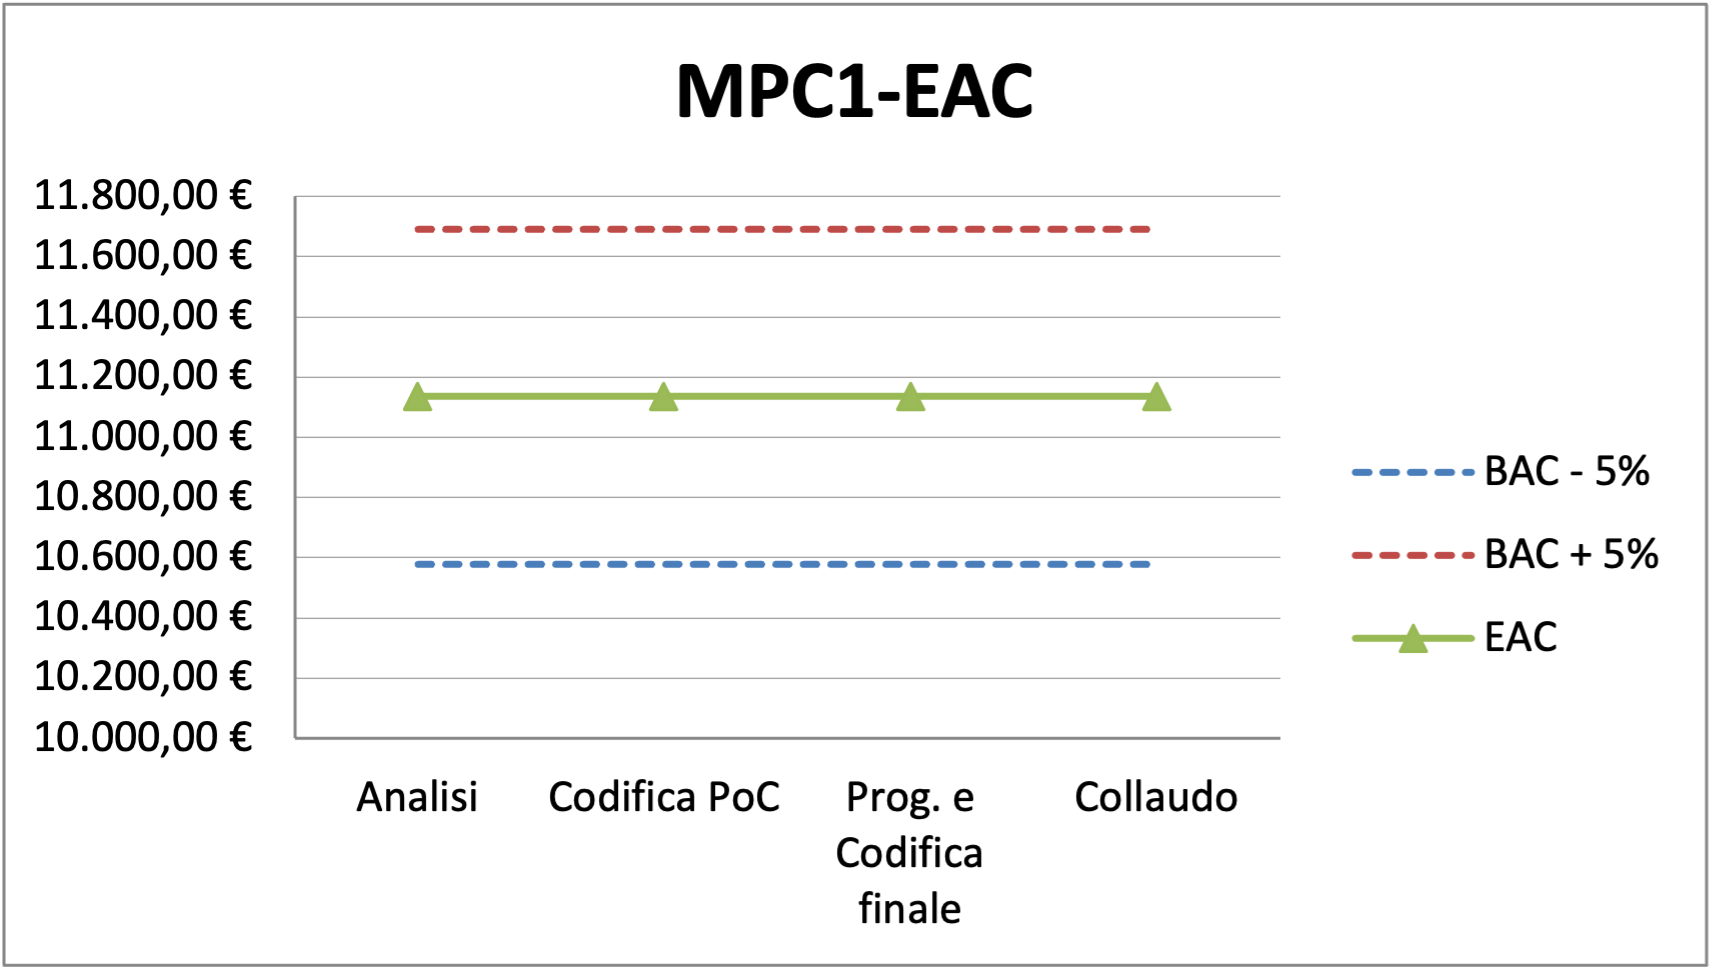
\includegraphics[width=0.8\textwidth]{images/MPC1-EAC.png}
    \caption{MPC1-EAC: Estimated At Completion}
\end{figure}
\noindent \textbf{Considerazioni RTB:} si nota come la stima del costo totale (EAC) sia in linea con il budget inizialmente preventivato per entrambi i periodi di Analisi e Codifica del PoC. Si vuole dunque cercare di mantenere questo risultato anche per i prossimi periodi.

\vspace{0.5cm}

\noindent \textbf{Considerazioni PB:} La stima del costo totale non ha mai subito variazioni nei periodi attraversati.

\newpage
\paragraph{MPC2-CV: Cost Variance}
\begin{figure}[h!] 
    \centering
    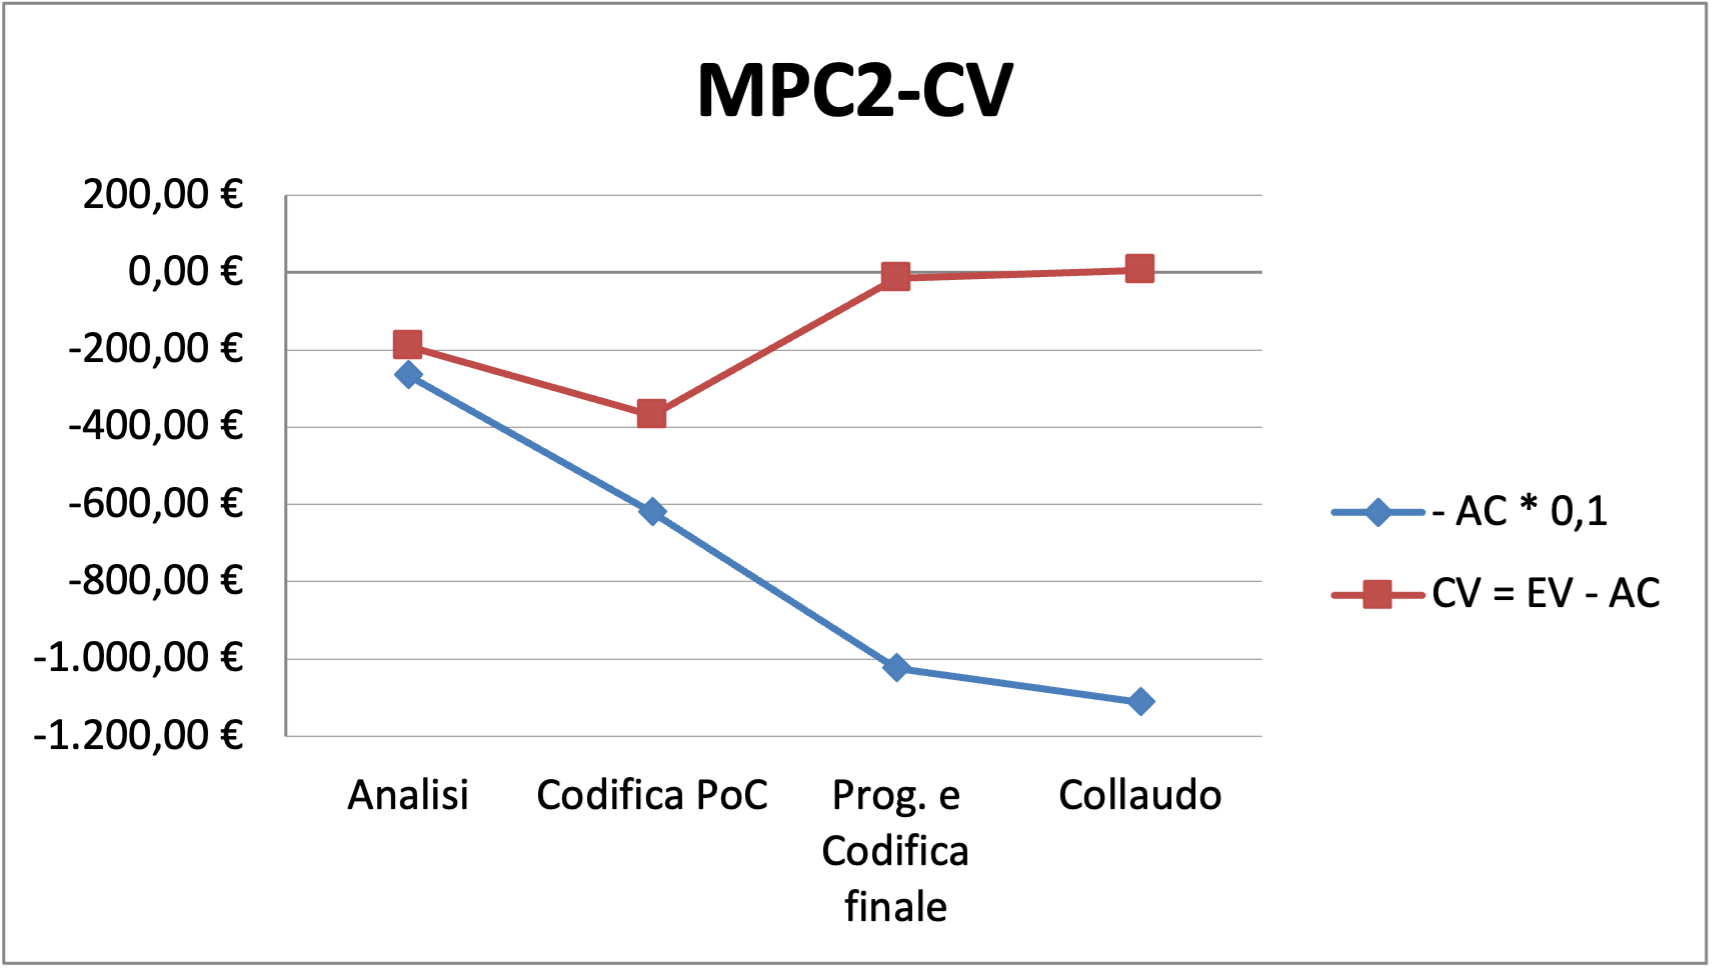
\includegraphics[width=0.8\textwidth]{images/MPC2-CV.png}
    \caption{MPC2-CV: Cost Variance}
\end{figure}
\noindent \textbf{Considerazioni RTB:} pur rimanendo entro i limiti previsti dalle metriche, il Cost Variance (CV) non rispetta il valore ottimale, in quanto il valore delle attività realizzate è inferiore al costo sostenuto. Sarà dunque necessario attuare dei miglioramenti dal punto di vista produttivo, in modo che i costi per le attività siano ben giustificati.

\paragraph{MPC3-SV: Schedule Variance}
\begin{figure}[h!]
    \centering
    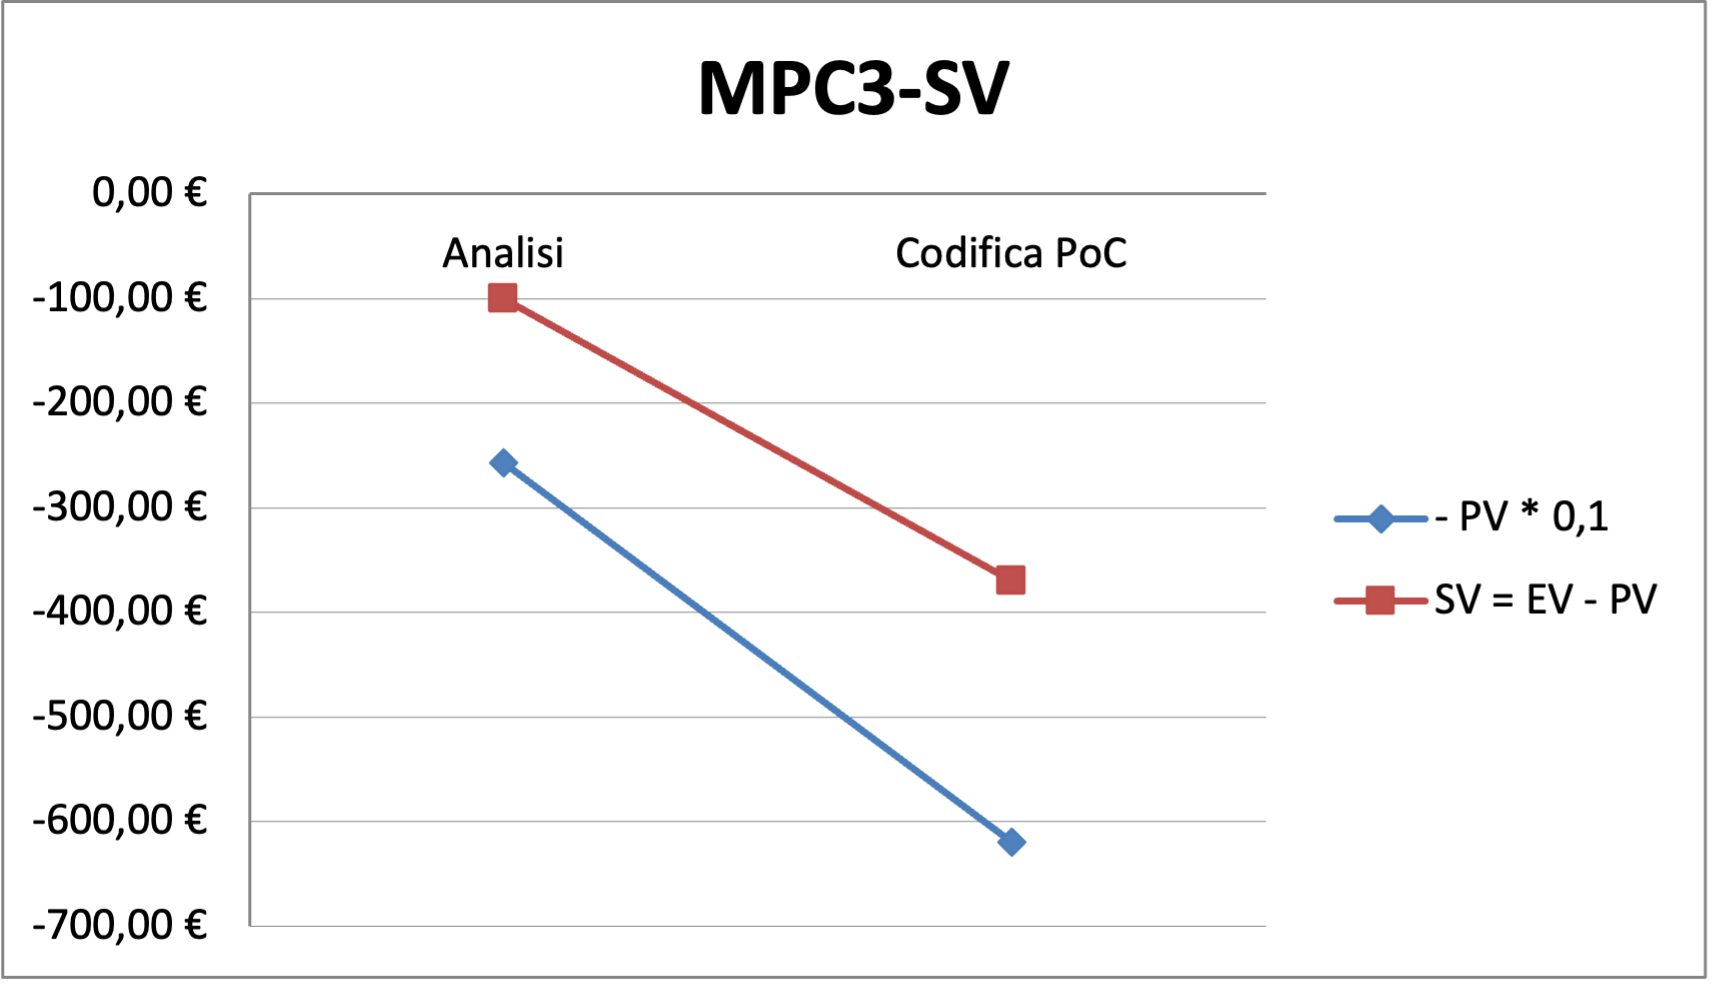
\includegraphics[width=0.8\textwidth]{images/MPC3-SV.png}
    \caption{MPC3-SV: Schedule Variance}
\end{figure}
\noindent \textbf{Considerazioni RTB:} si nota come la Schedule Variance (SV) risulta avere un calo durante il periodo di progettazione e codifica del PoC, suggerendo quindi che ci sono stati dei ritardi rispetto alla pianificazione prevista. Il motivo di questi ritardi è dovuto allo studio delle nuove tecnologie che ha richiesto più tempo del previsto e alla sessione di esami che ha tolto del tempo allo svolgimento del progetto.

\newpage
\paragraph{MPC4-BV: Budget Variance}
\begin{figure}[h!] 
    \centering
    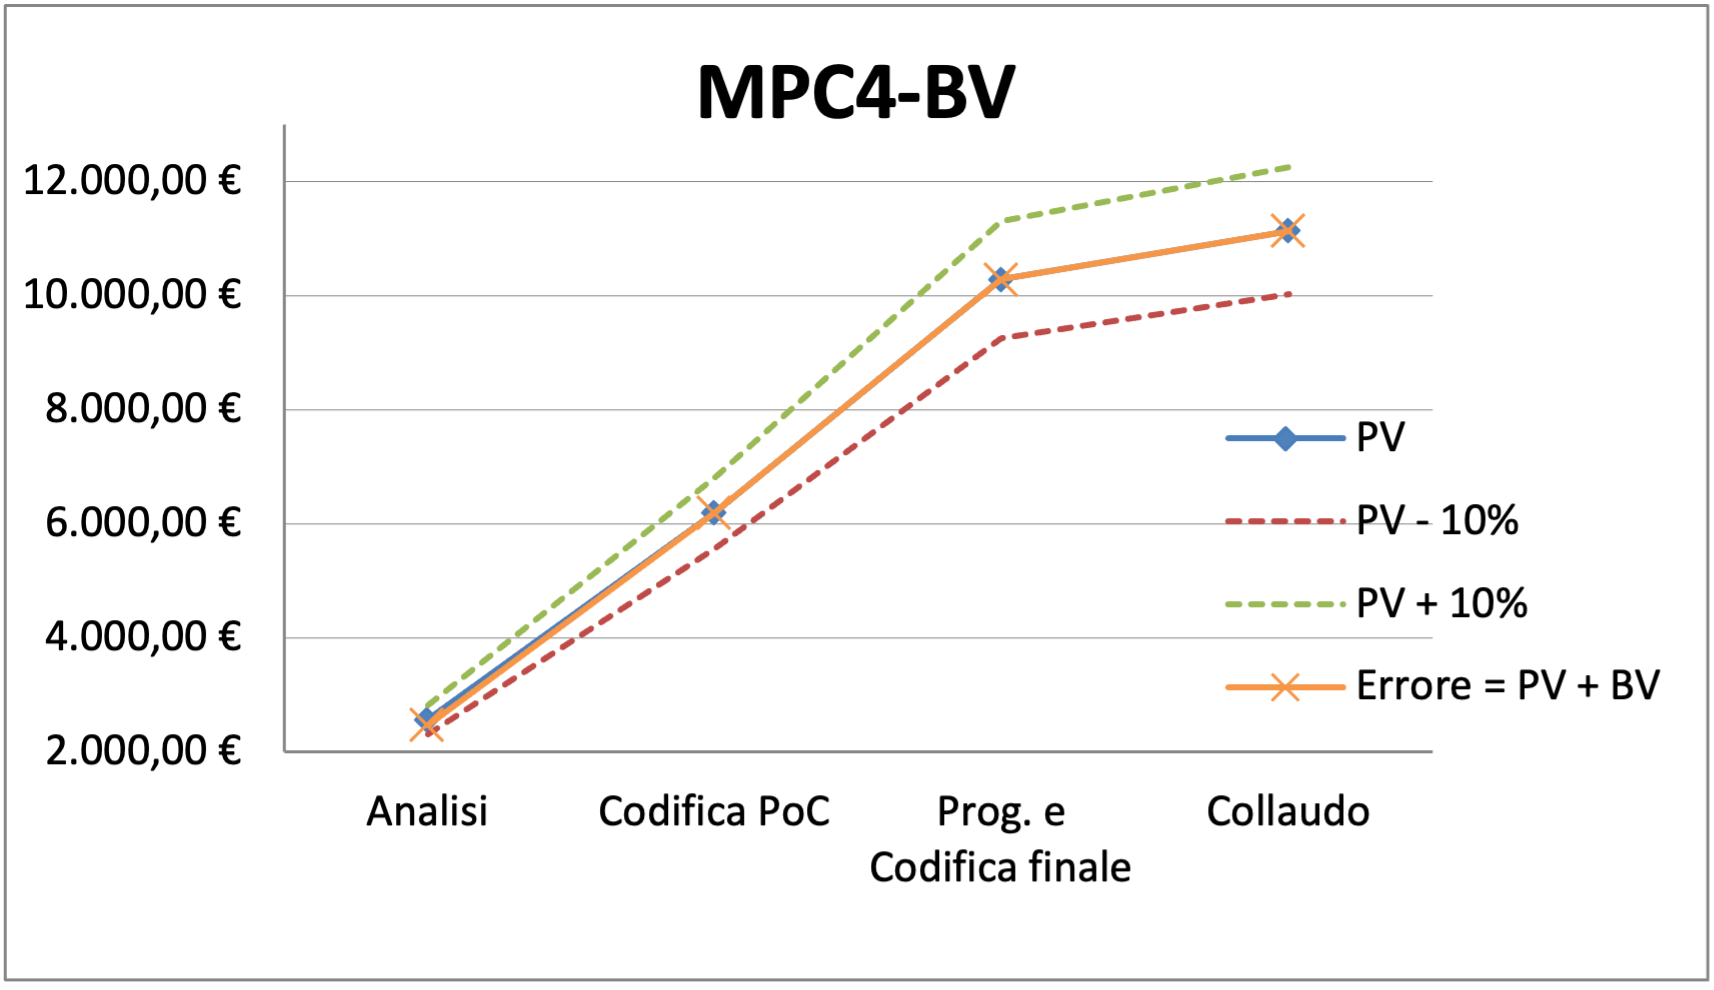
\includegraphics[width=0.8\textwidth]{images/MPC4-BV.png}
    \caption{MPC4-BV: Budget Variance}
\end{figure}
\noindent \textbf{Considerazioni RTB:} si nota come sostanzialmente l'errore rimane pressoché nullo, a significare che i costi della pianificazione iniziale corrispondono quasi completamente a quelli effettivi. Si cerca di dunque di mantenere questa linea anche per i prossimi periodi.

\paragraph{MPC5-PV: Planned Value}
\begin{figure}[h!]
    \centering
    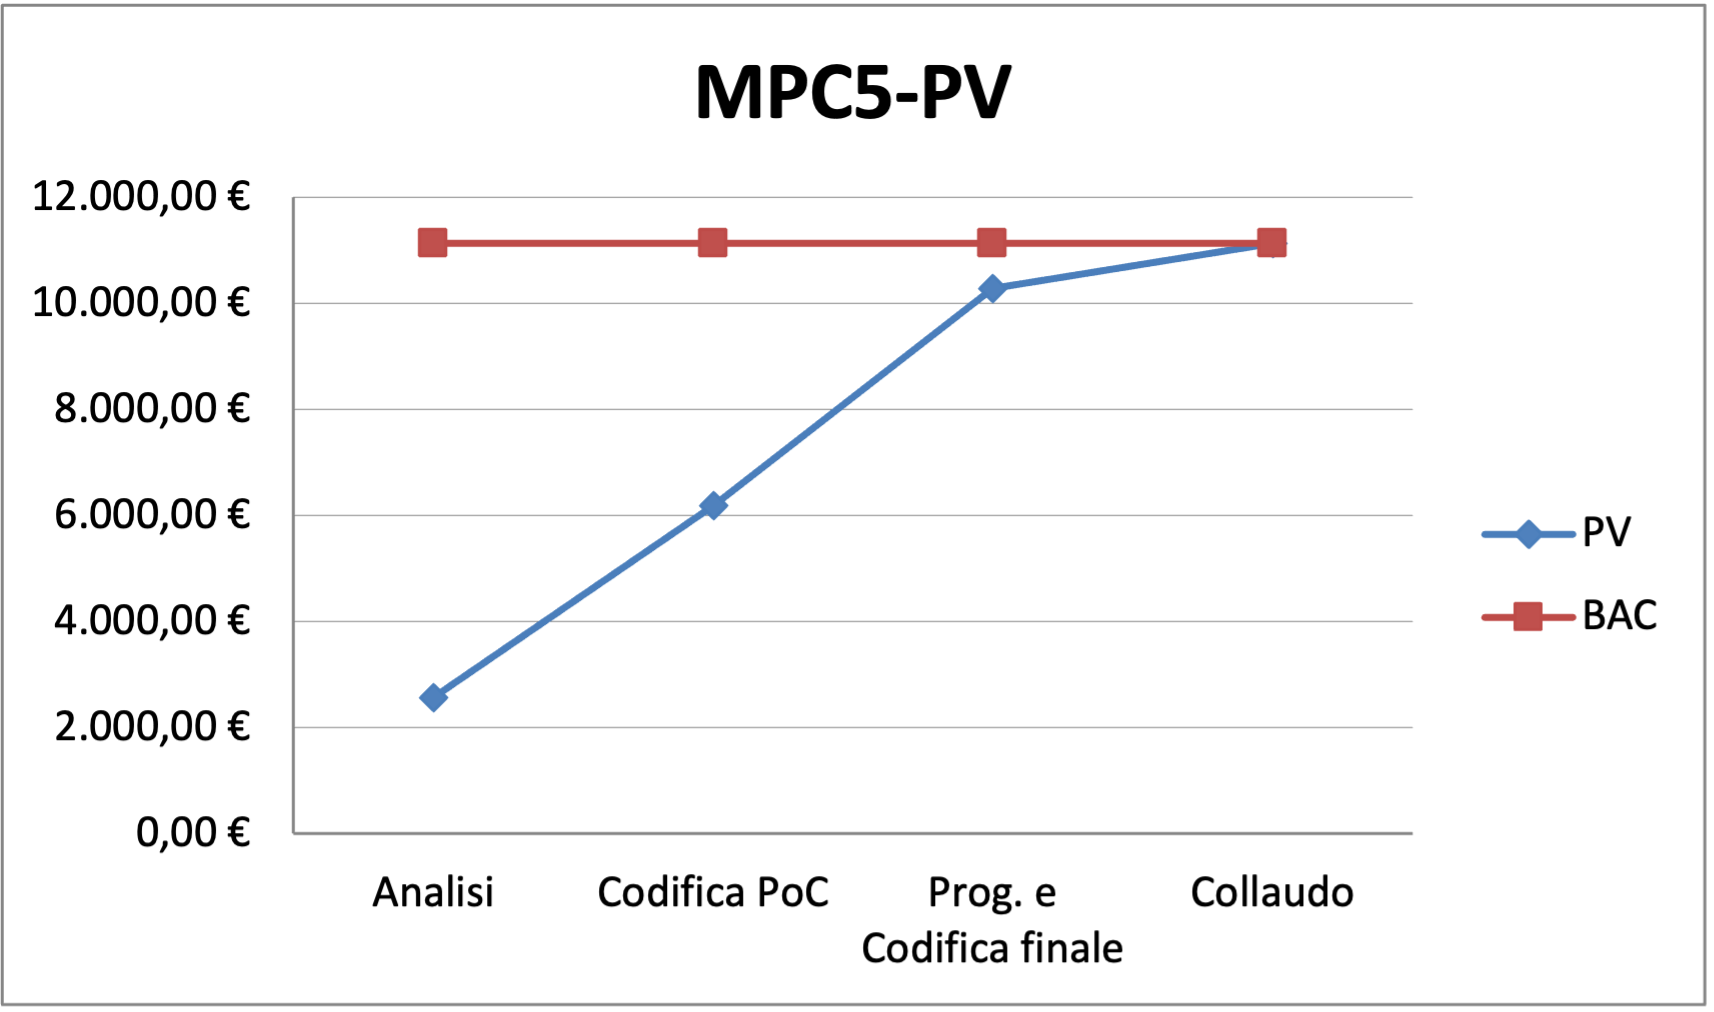
\includegraphics[width=0.8\textwidth]{images/MPC5-PV.png}
    \caption{MPC5-PV: Planned Value}
\end{figure}
\noindent \textbf{Considerazioni RTB:} si deduce dal grafico che i costi sostenuti per i periodi di Analisi e Codifica del PoC rimangono inferiori a quelli previsti totalmente per la realizzazione del progetto. Ovviamente si ha un incremento in questi costi dovuti all'avanzare del progetto, ma rimane comunque controllato.

\newpage

\noindent \textbf{Considerazioni PB:} 
\begin{itemize}
    \item \textbf{Progettazione:} Si prevede un medio consumo di risorse per questa fase, in linea con le aspettative. Non sono necessarie azioni risanatorie.
    \item \textbf{Codifica MVP:} Per questa fase si prevede un sostanziale consumo di risorse, in linea con le aspettative. Non sono necessarie azioni risanatorie
    \item \textbf{Progettazione:} Il budget rimanente scarseggia ma la previsione finale si allinea a quella iniziale. 
\end{itemize}

\paragraph{MPC6-AC: Actual Cost}
\begin{figure}[h!] 
    \centering
    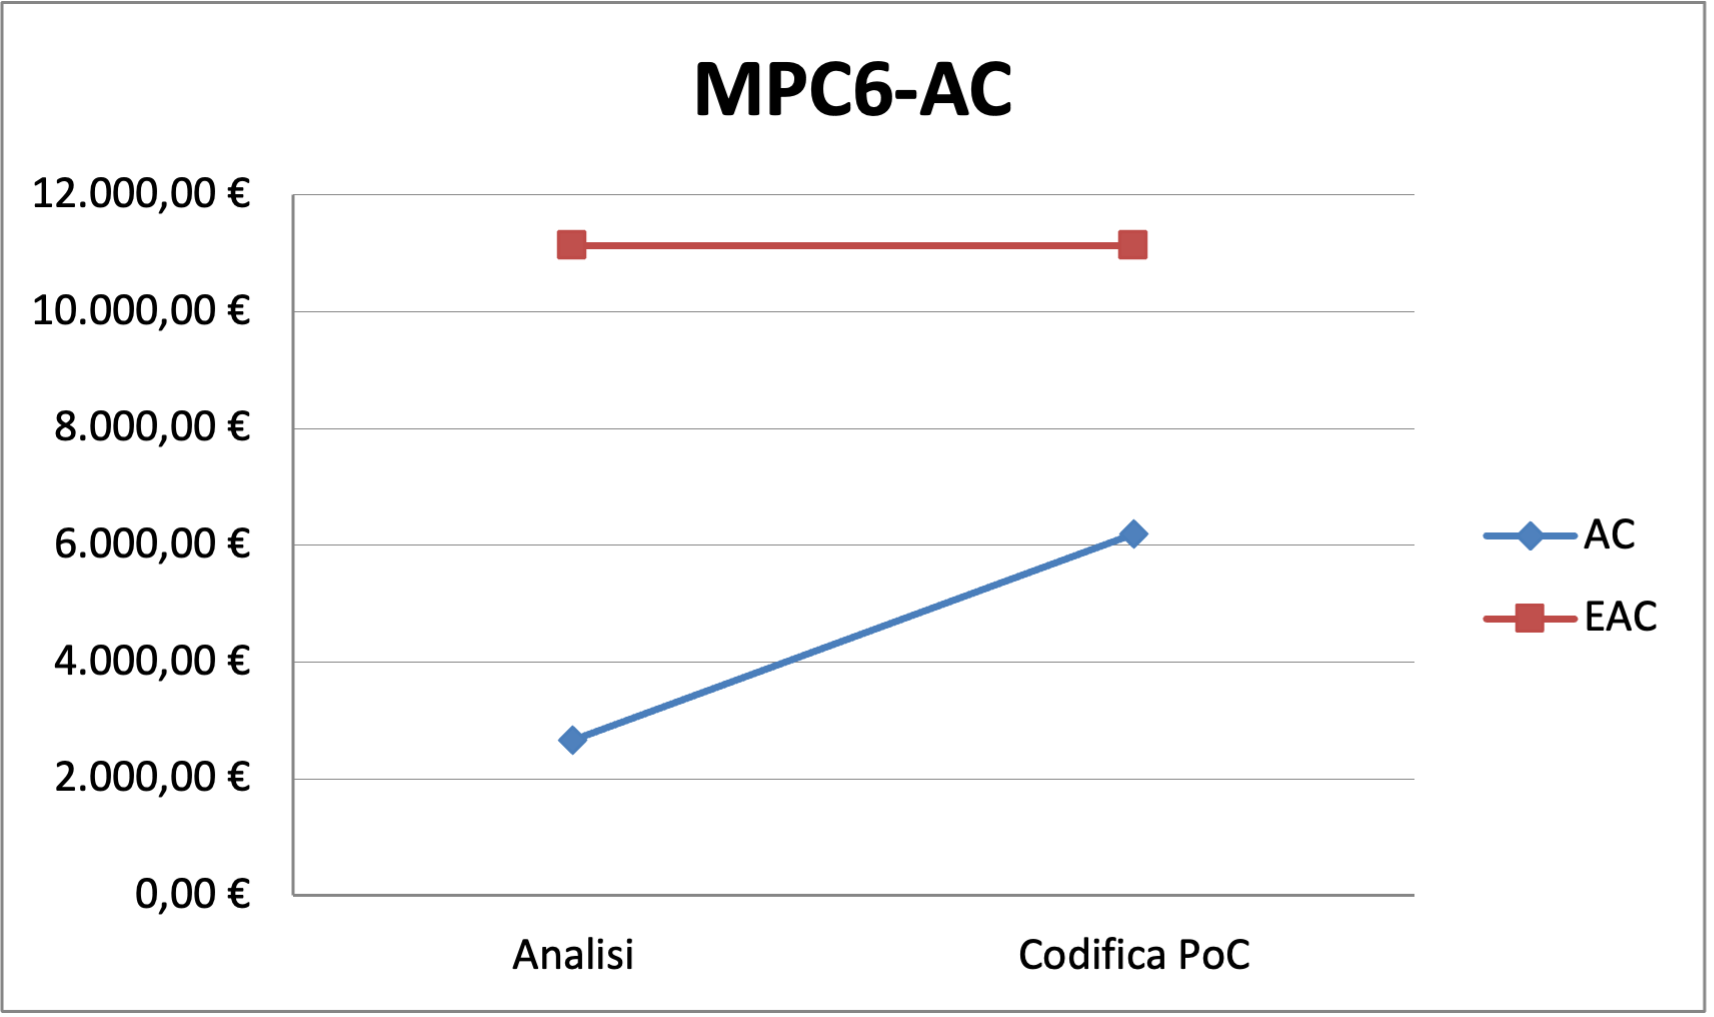
\includegraphics[width=0.8\textwidth]{images/MPC6-AC.png}
    \caption{MPC6-AC: Actual Cost}
\end{figure}
\noindent \textbf{Considerazioni RTB:} si osserva che l’Actual Cost (AC) mostra un incremento, come naturale con il progredire del progetto, ma rimane comunque sotto la soglia dell'Estimated at Completion (EAC). 

\paragraph{MPC7-EV: Earned Value}
\begin{figure}[h!] 
    \centering
    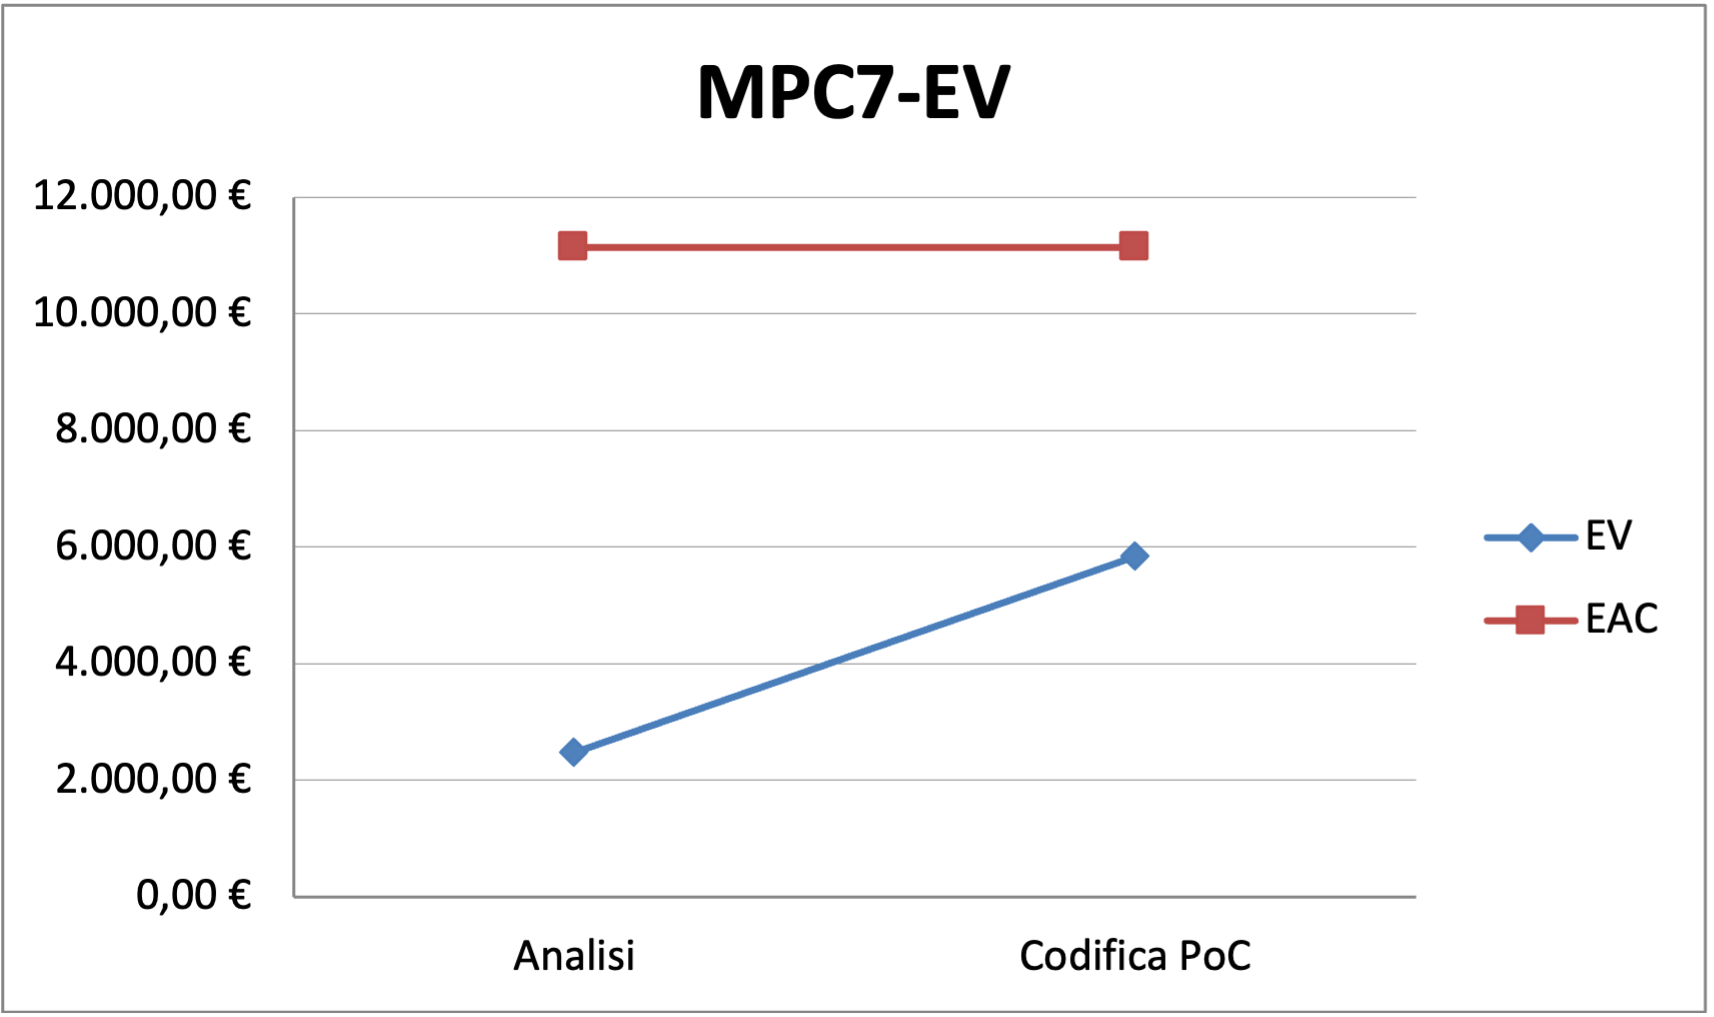
\includegraphics[width=0.8\textwidth]{images/MPC7-EV.png}
    \caption{MPC7-EV: Earned Value}
\end{figure}
\noindent \textbf{Considerazioni RTB:} si nota che l'Earned Value (EV) rimane minore dell'Estimated at Completion (EAC), a significare che il valore effettivo delle attività di progetto svolte fino all'RTB non sfora i costi pianificati per l'intero progetto, seppur ovviamente aumenta con il susseguirsi dei vari periodi.

\subsubsection{Sviluppo} \label{sec:sviluppo}
\paragraph{MPC8-SFINp}
\subsection{Processi di supporto} \label{sec:processi_di_supporto}
Di seguito sono visualizzati i grafici relativi alle metriche dei processi di supporto.
\subsubsection{Qualità di processo - Documentazione}
\paragraph{MPC13-EOD: Errori ortografici per documento}
\begin{figure}[h!] 
    \centering
    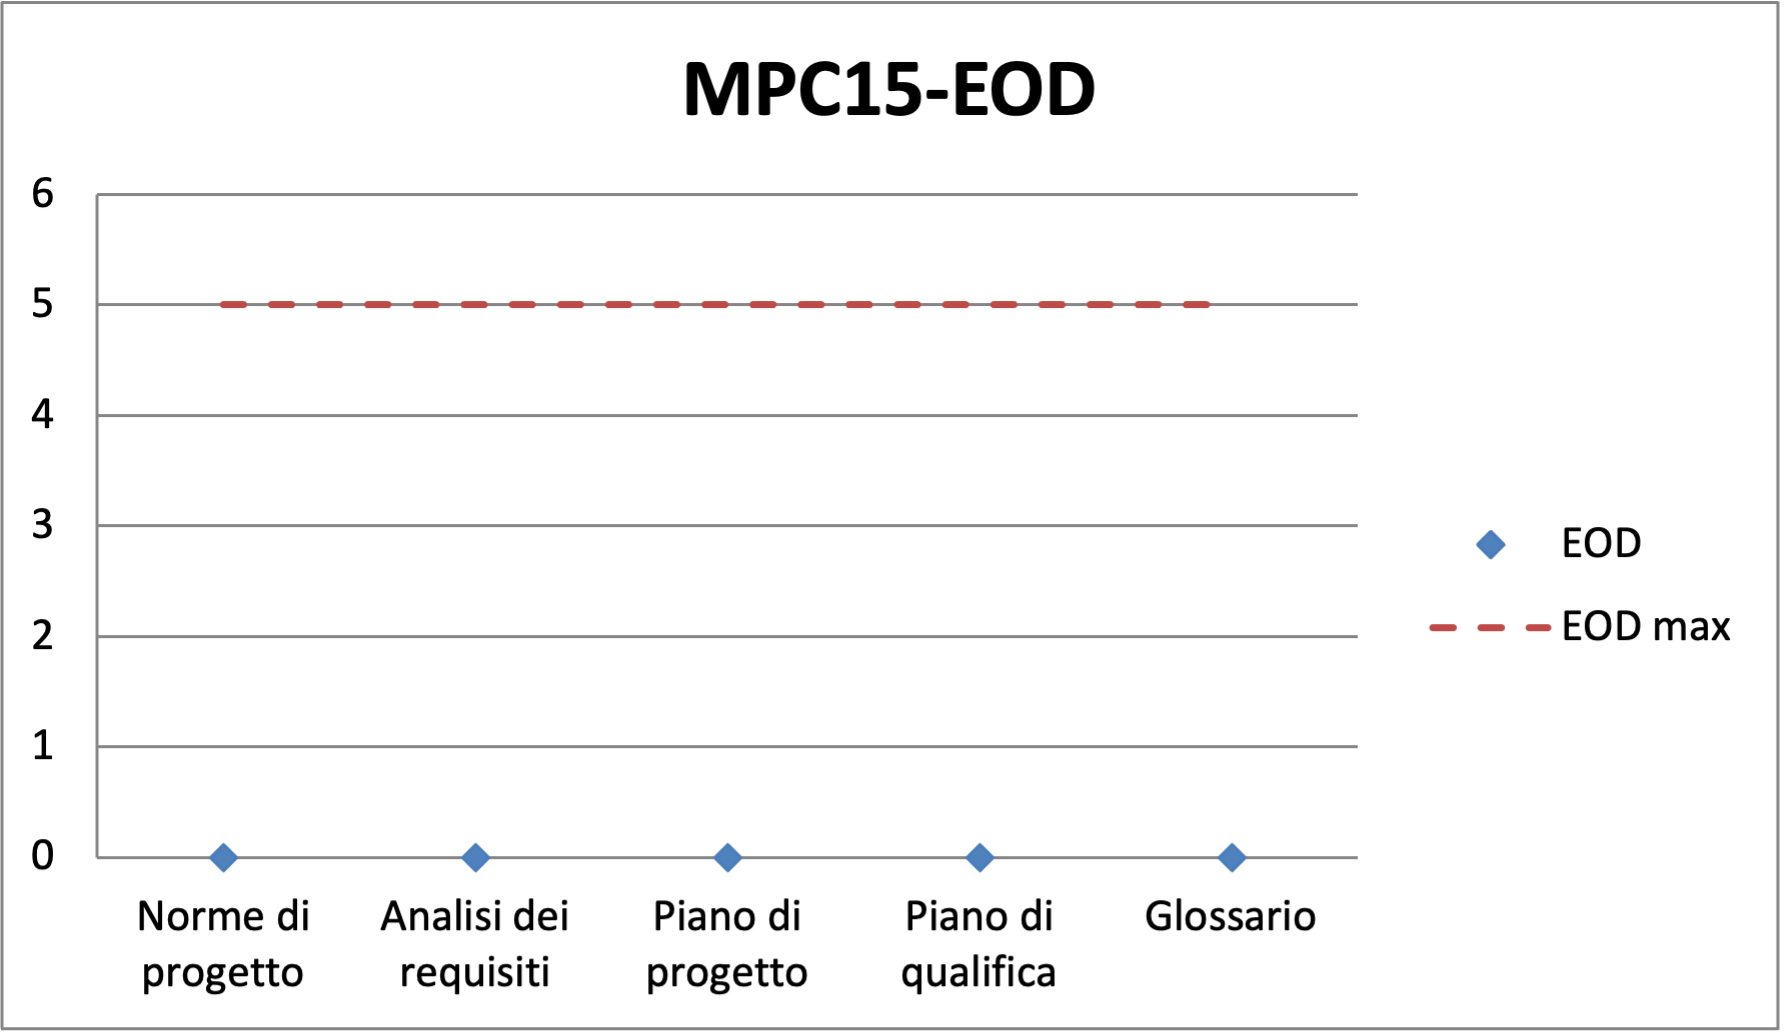
\includegraphics[width=0.8\textwidth]{images/MPC13-EOD.png}
    \caption{MPC13-EOD: Errori ortografici per documento}
\end{figure}
\noindent \textbf{Considerazioni RTB:} si osserva che non sono presenti errori ortografici in nessun documento. Pertanto, si ha un valore ottimale per quanto riguarda questa metrica (MPC13-EOD). Ciò significa che il gruppo ha prestato una particolare attenzione alla correttezza ortografica dei documenti.


\paragraph{MPC14-IG: Indice Gulpease}
\begin{figure}[h!] 
    \centering
    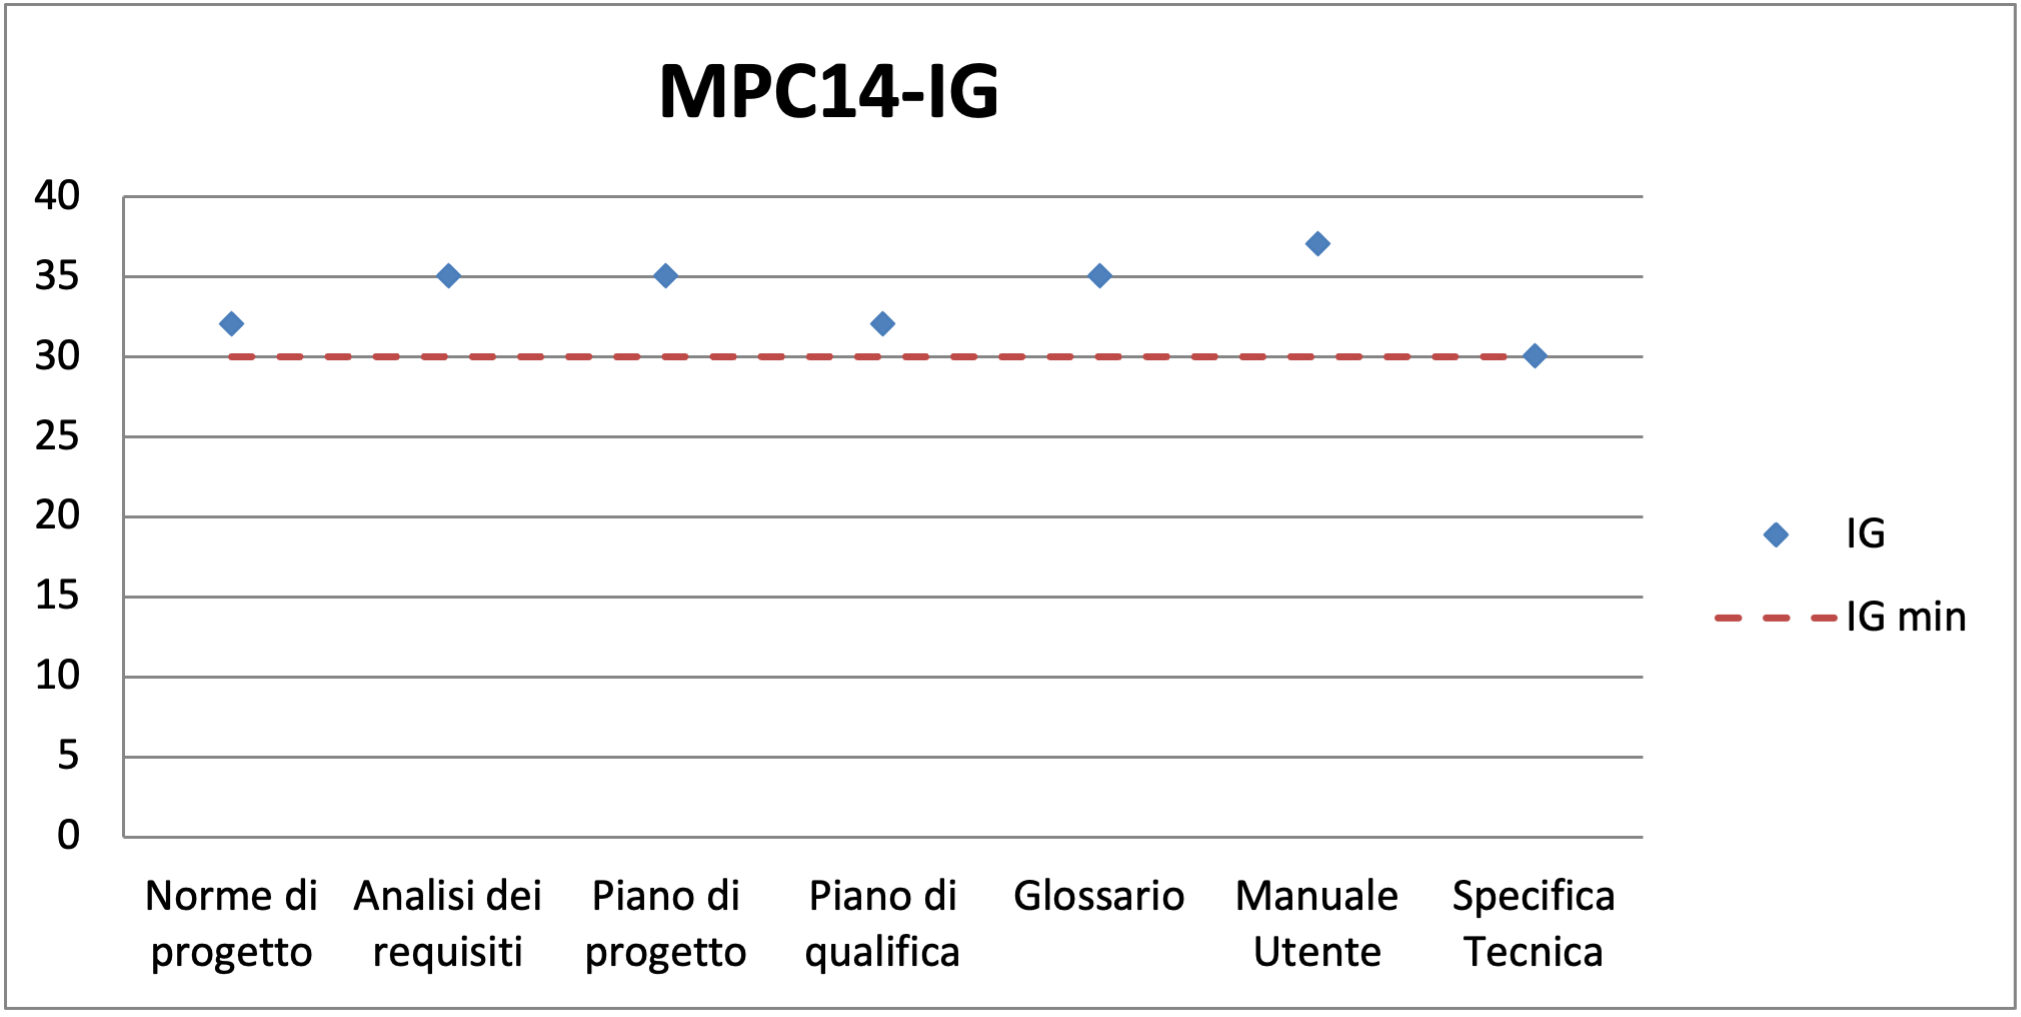
\includegraphics[width=0.8\textwidth]{images/MPC14-IG.png}
    \caption{MPC14-IG: Indice Gulpease}
\end{figure}
\noindent \textbf{Considerazioni RTB:} si osserva come l'indice di Gulpease rimane accettabile per tutti i documenti, tuttavia non raggiunge mai l'ottimalità. Il gruppo, pertanto, dovrà impegnarsi ad utilizzare termini meno tecnici (se possibile) e strutturare i periodi in maniera più semplice.

\subsubsection{Qualità di processo - Accertamento della qualità}
\paragraph{MPC15-MS: Metriche soddisfatte} \label{sec:accertamento delle qualita}
\noindent \textbf{Considerazioni RTB:}
le metriche prese in considerazione in questa fase sono:
\begin{itemize}
    \item MPC1-EAC \colorbox{green}{Soddisfatta};
    \item MPC2-CV \colorbox{green}{Soddisfatta};
    \item MPC3-SV \colorbox{green}{Soddisfatta};
    \item MPC4-BV \colorbox{green}{Soddisfatta};
    \item MPC5-PV \colorbox{green}{Soddisfatta};
    \item MPC6-AC \colorbox{green}{Soddisfatta};
    \item MPC7-EV \colorbox{green}{Soddisfatta};
    \item MPC13-EOD \colorbox{green}{Soddisfatta};
    \item MPC14-IG \colorbox{green}{Soddisfatta}.
\end{itemize}
\noindent La percentuale di metriche soddisfatte (MPC15-MS) equivale al \textbf{100\%}. Pertanto, possiamo dire che si è raggiunto un livello di ottimalità per questa metrica.

\newpage
\subsection{Qualità di prodotto}
\subsubsection{Portabilità su altre piattaforme}
\paragraph{Google Chrome}
\begin{figure}[h!] 
    \centering
    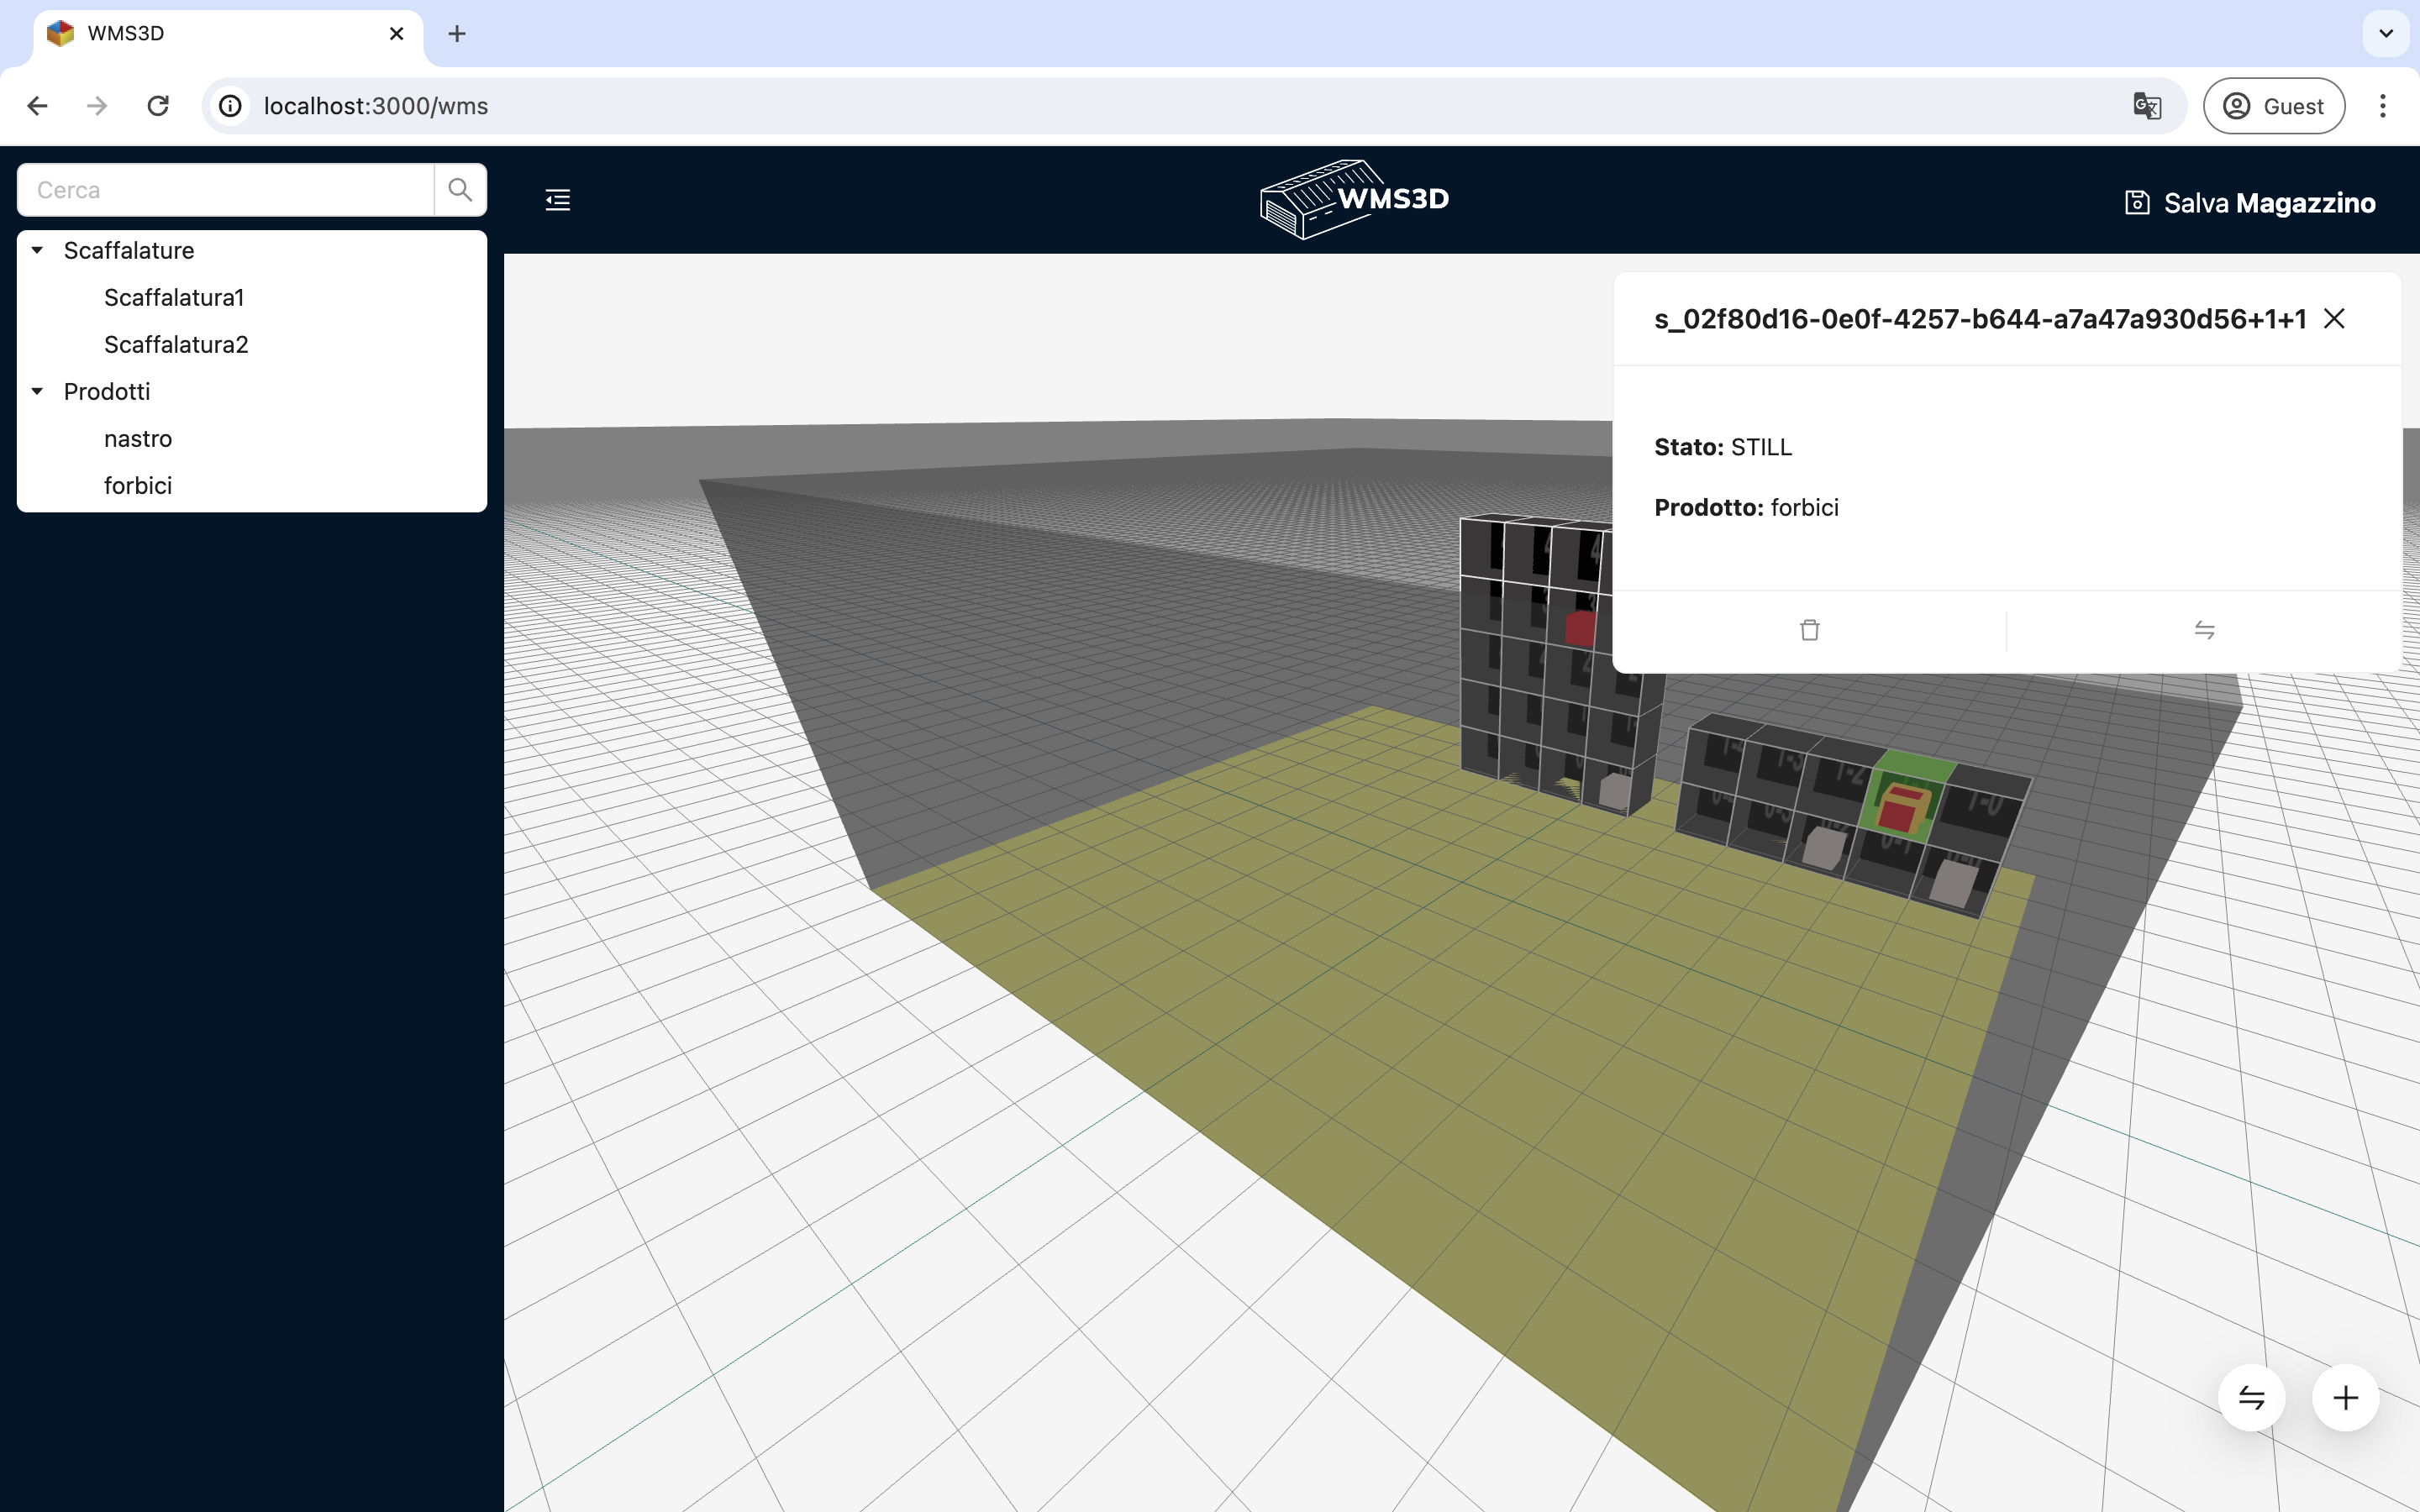
\includegraphics[width=0.8\textwidth]{images/chrome.png}
    \caption{Test su Google Chrome}
\end{figure}
Versione: 124.0.6367.119 (Official Build) (arm64)

\paragraph{Safari}
\begin{figure}[h!] 
    \centering
    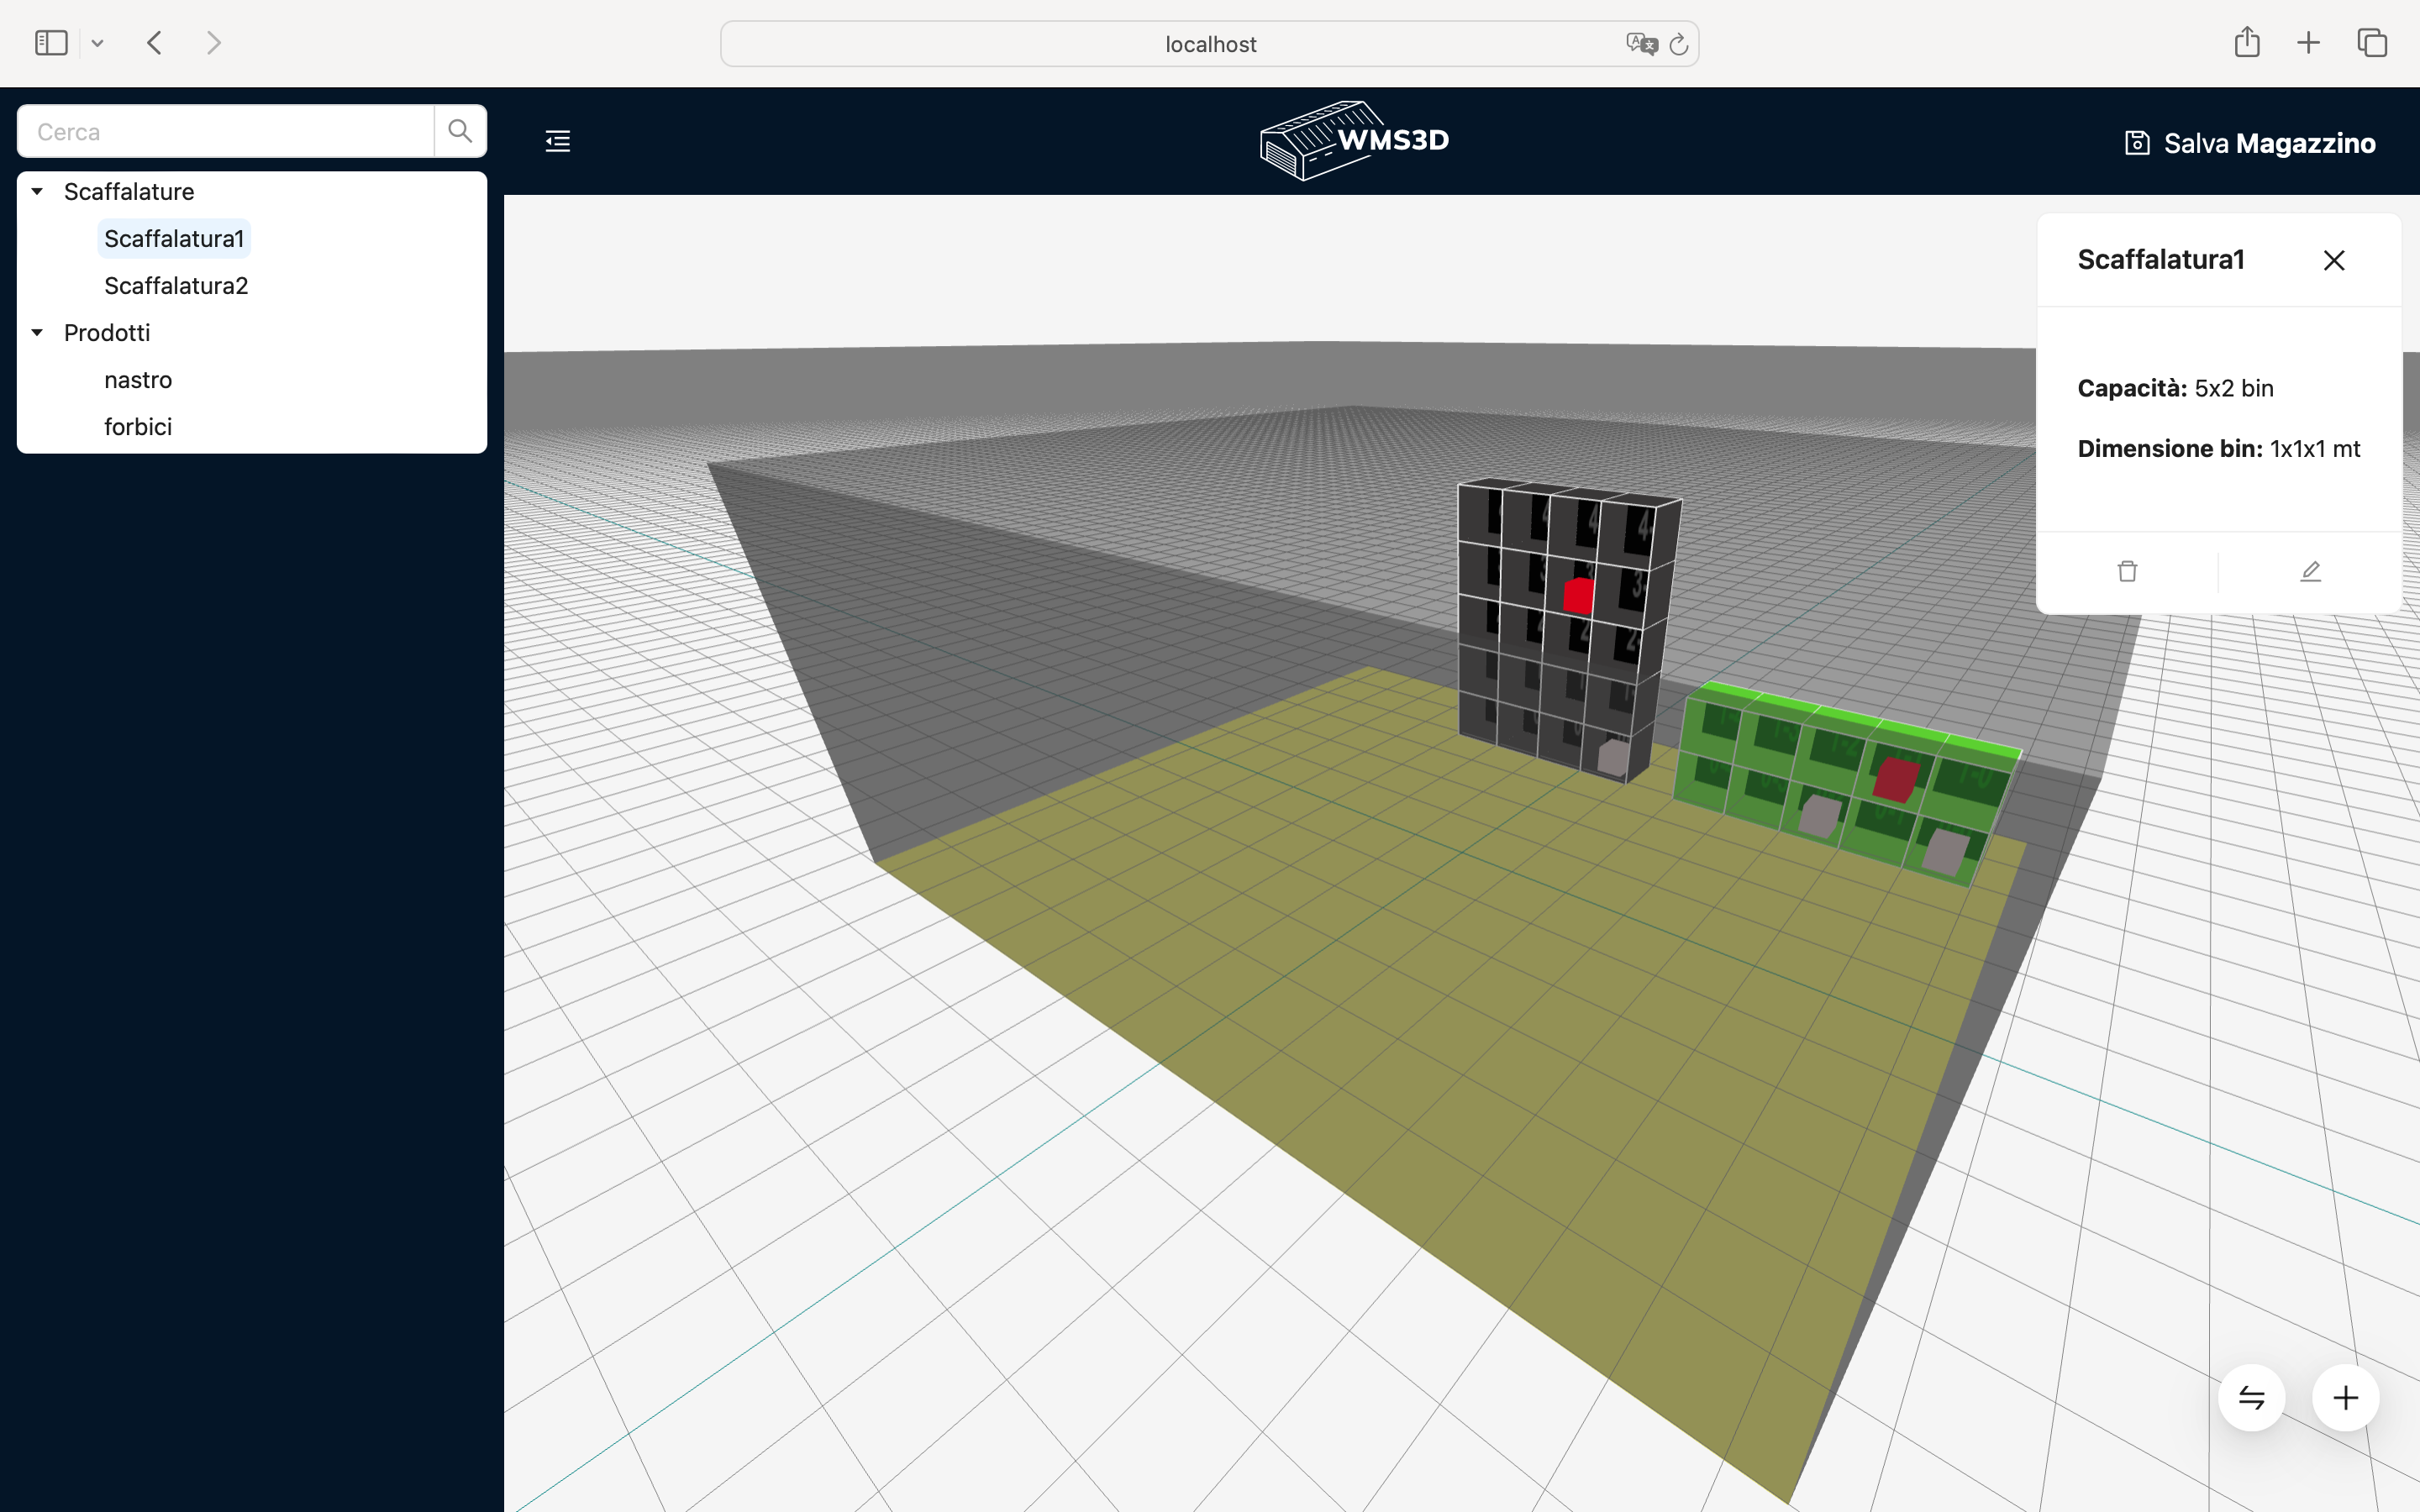
\includegraphics[width=0.8\textwidth]{images/safari.png}
    \caption{Test su Safari}
\end{figure}
Versione: 17.1.2 (19616.2.9.11.12)


\paragraph{Firefox}
\begin{figure}[h!] 
    \centering
    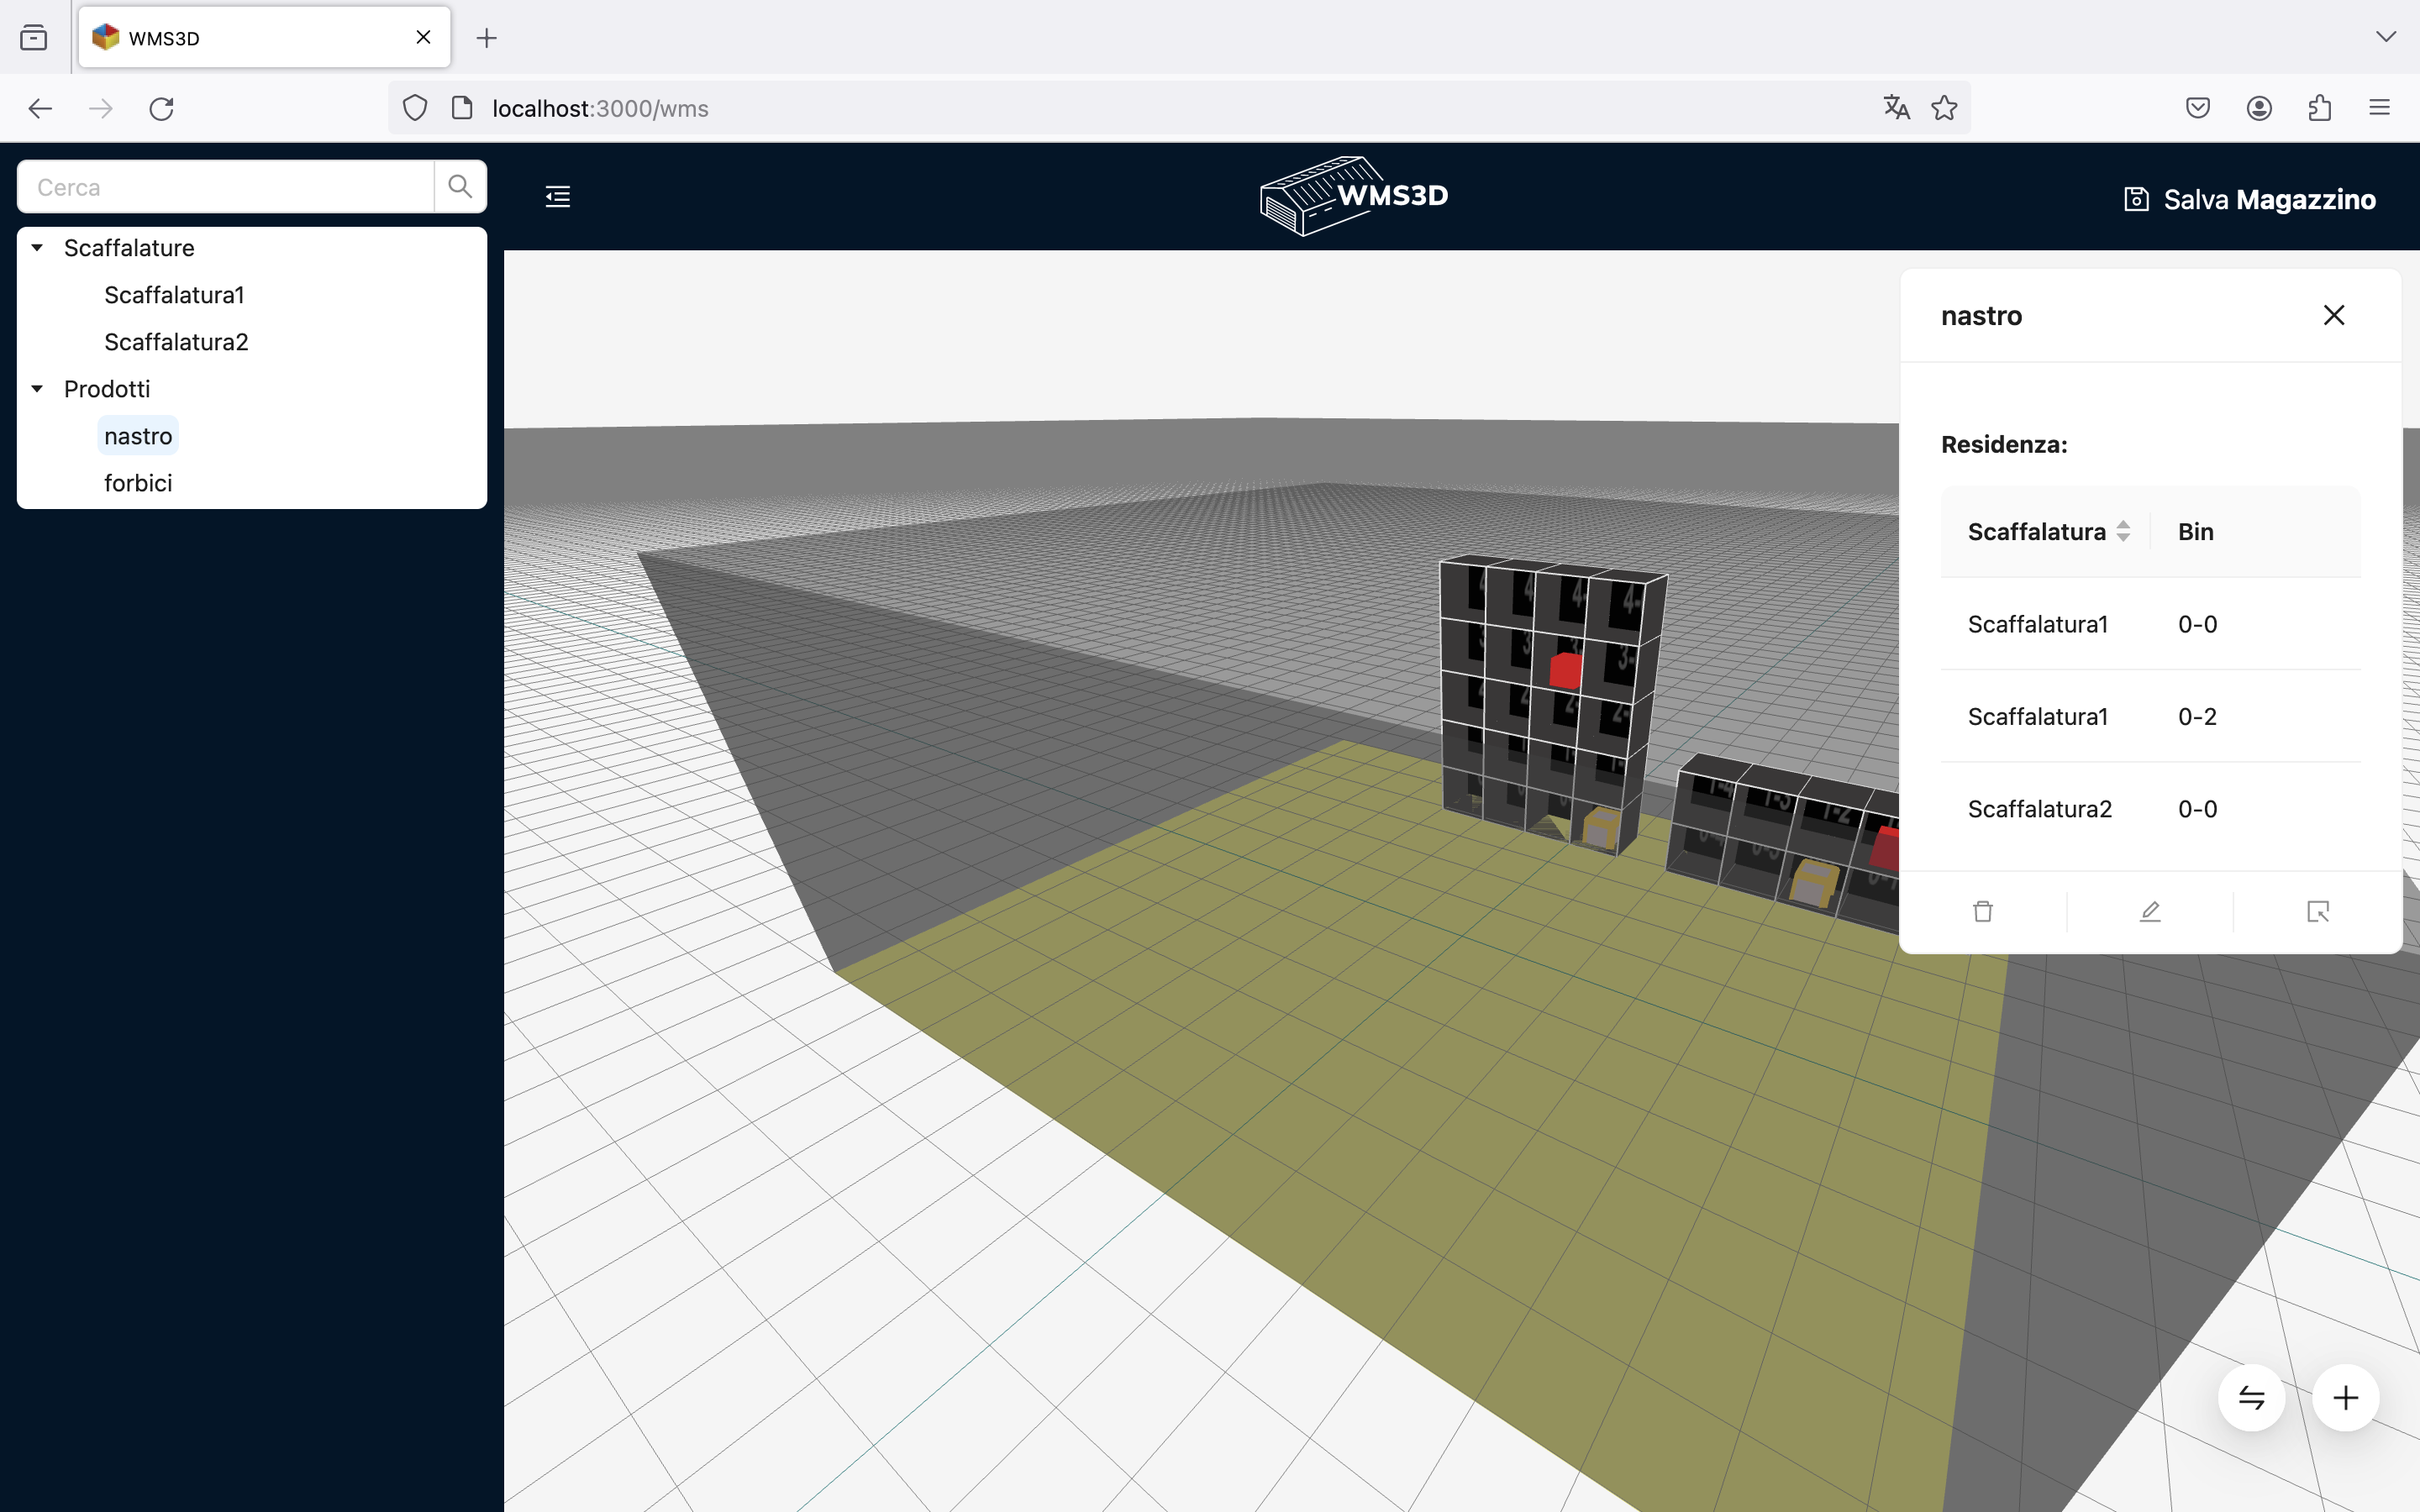
\includegraphics[width=0.8\textwidth]{images/firefox.png}
    \caption{Test su Firefox}
\end{figure}
Versione: 115 (64-bit)

\paragraph{Opera}
\begin{figure}[h!] 
    \centering
    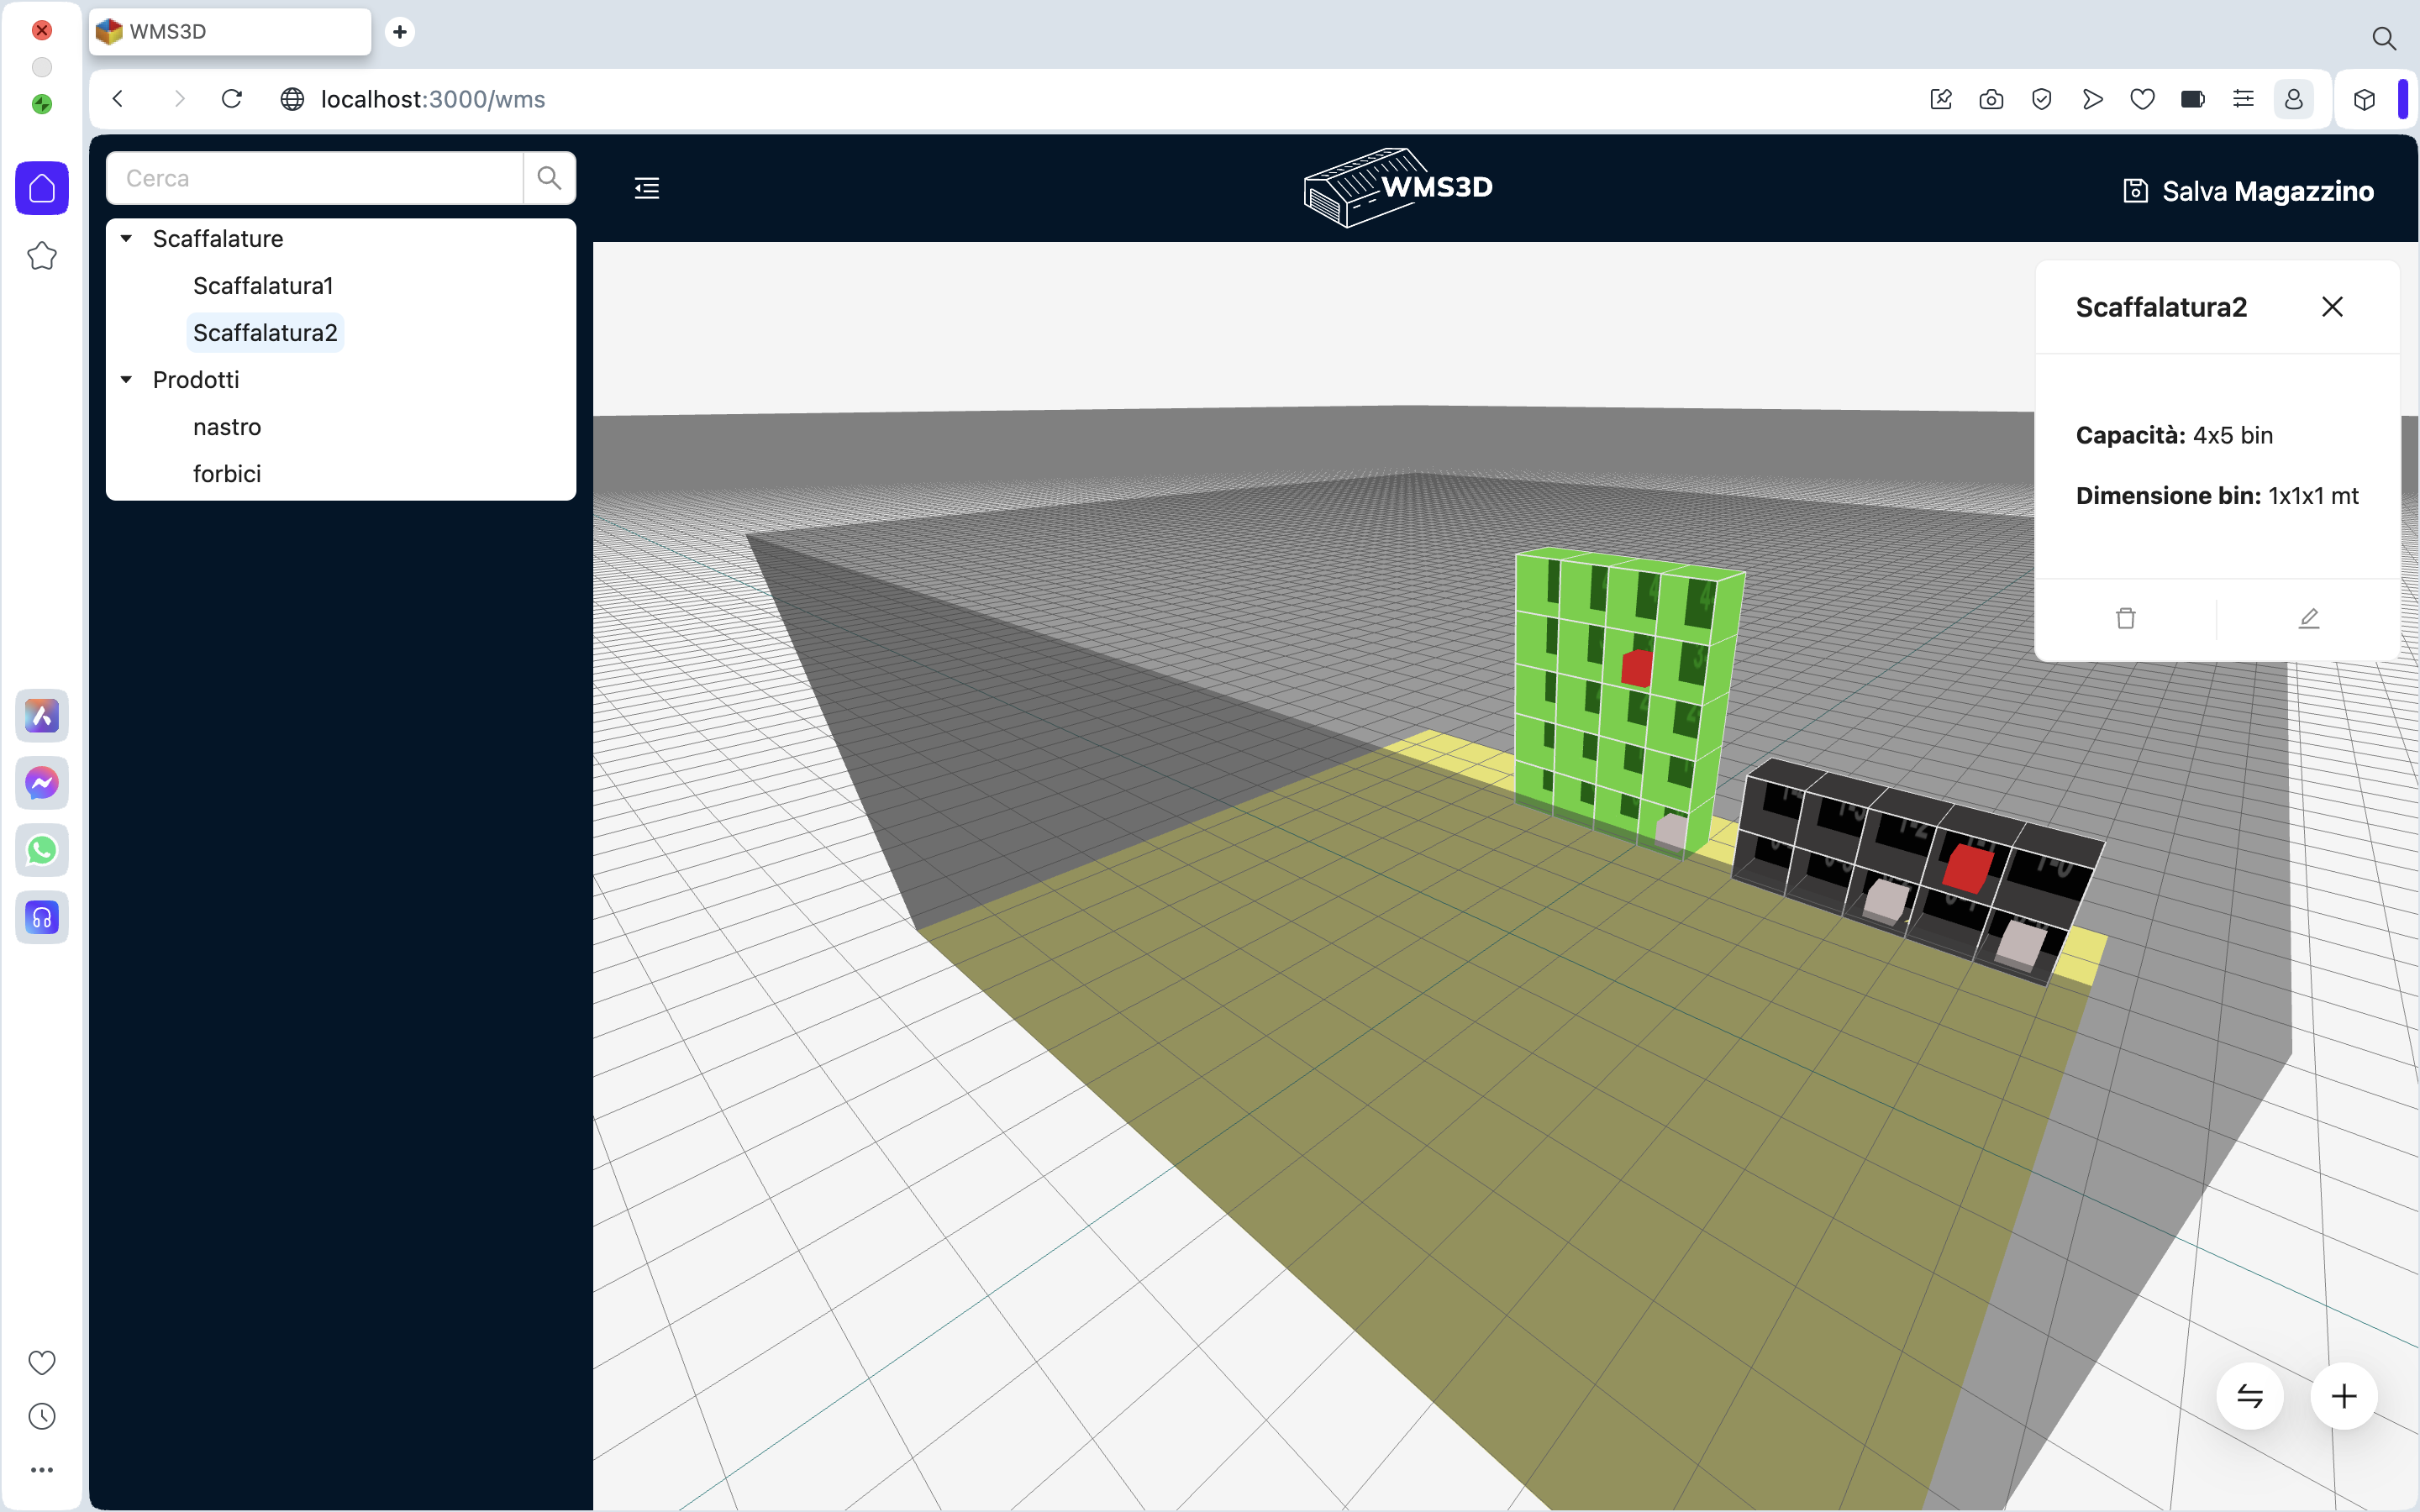
\includegraphics[width=0.8\textwidth]{images/opera.png}
    \caption{Test su Opera}
\end{figure}
Versione: 109.0.5097.68 (arm64)

\newpage

\paragraph{Microsoft Edge}
\begin{figure}[h!] 
    \centering
    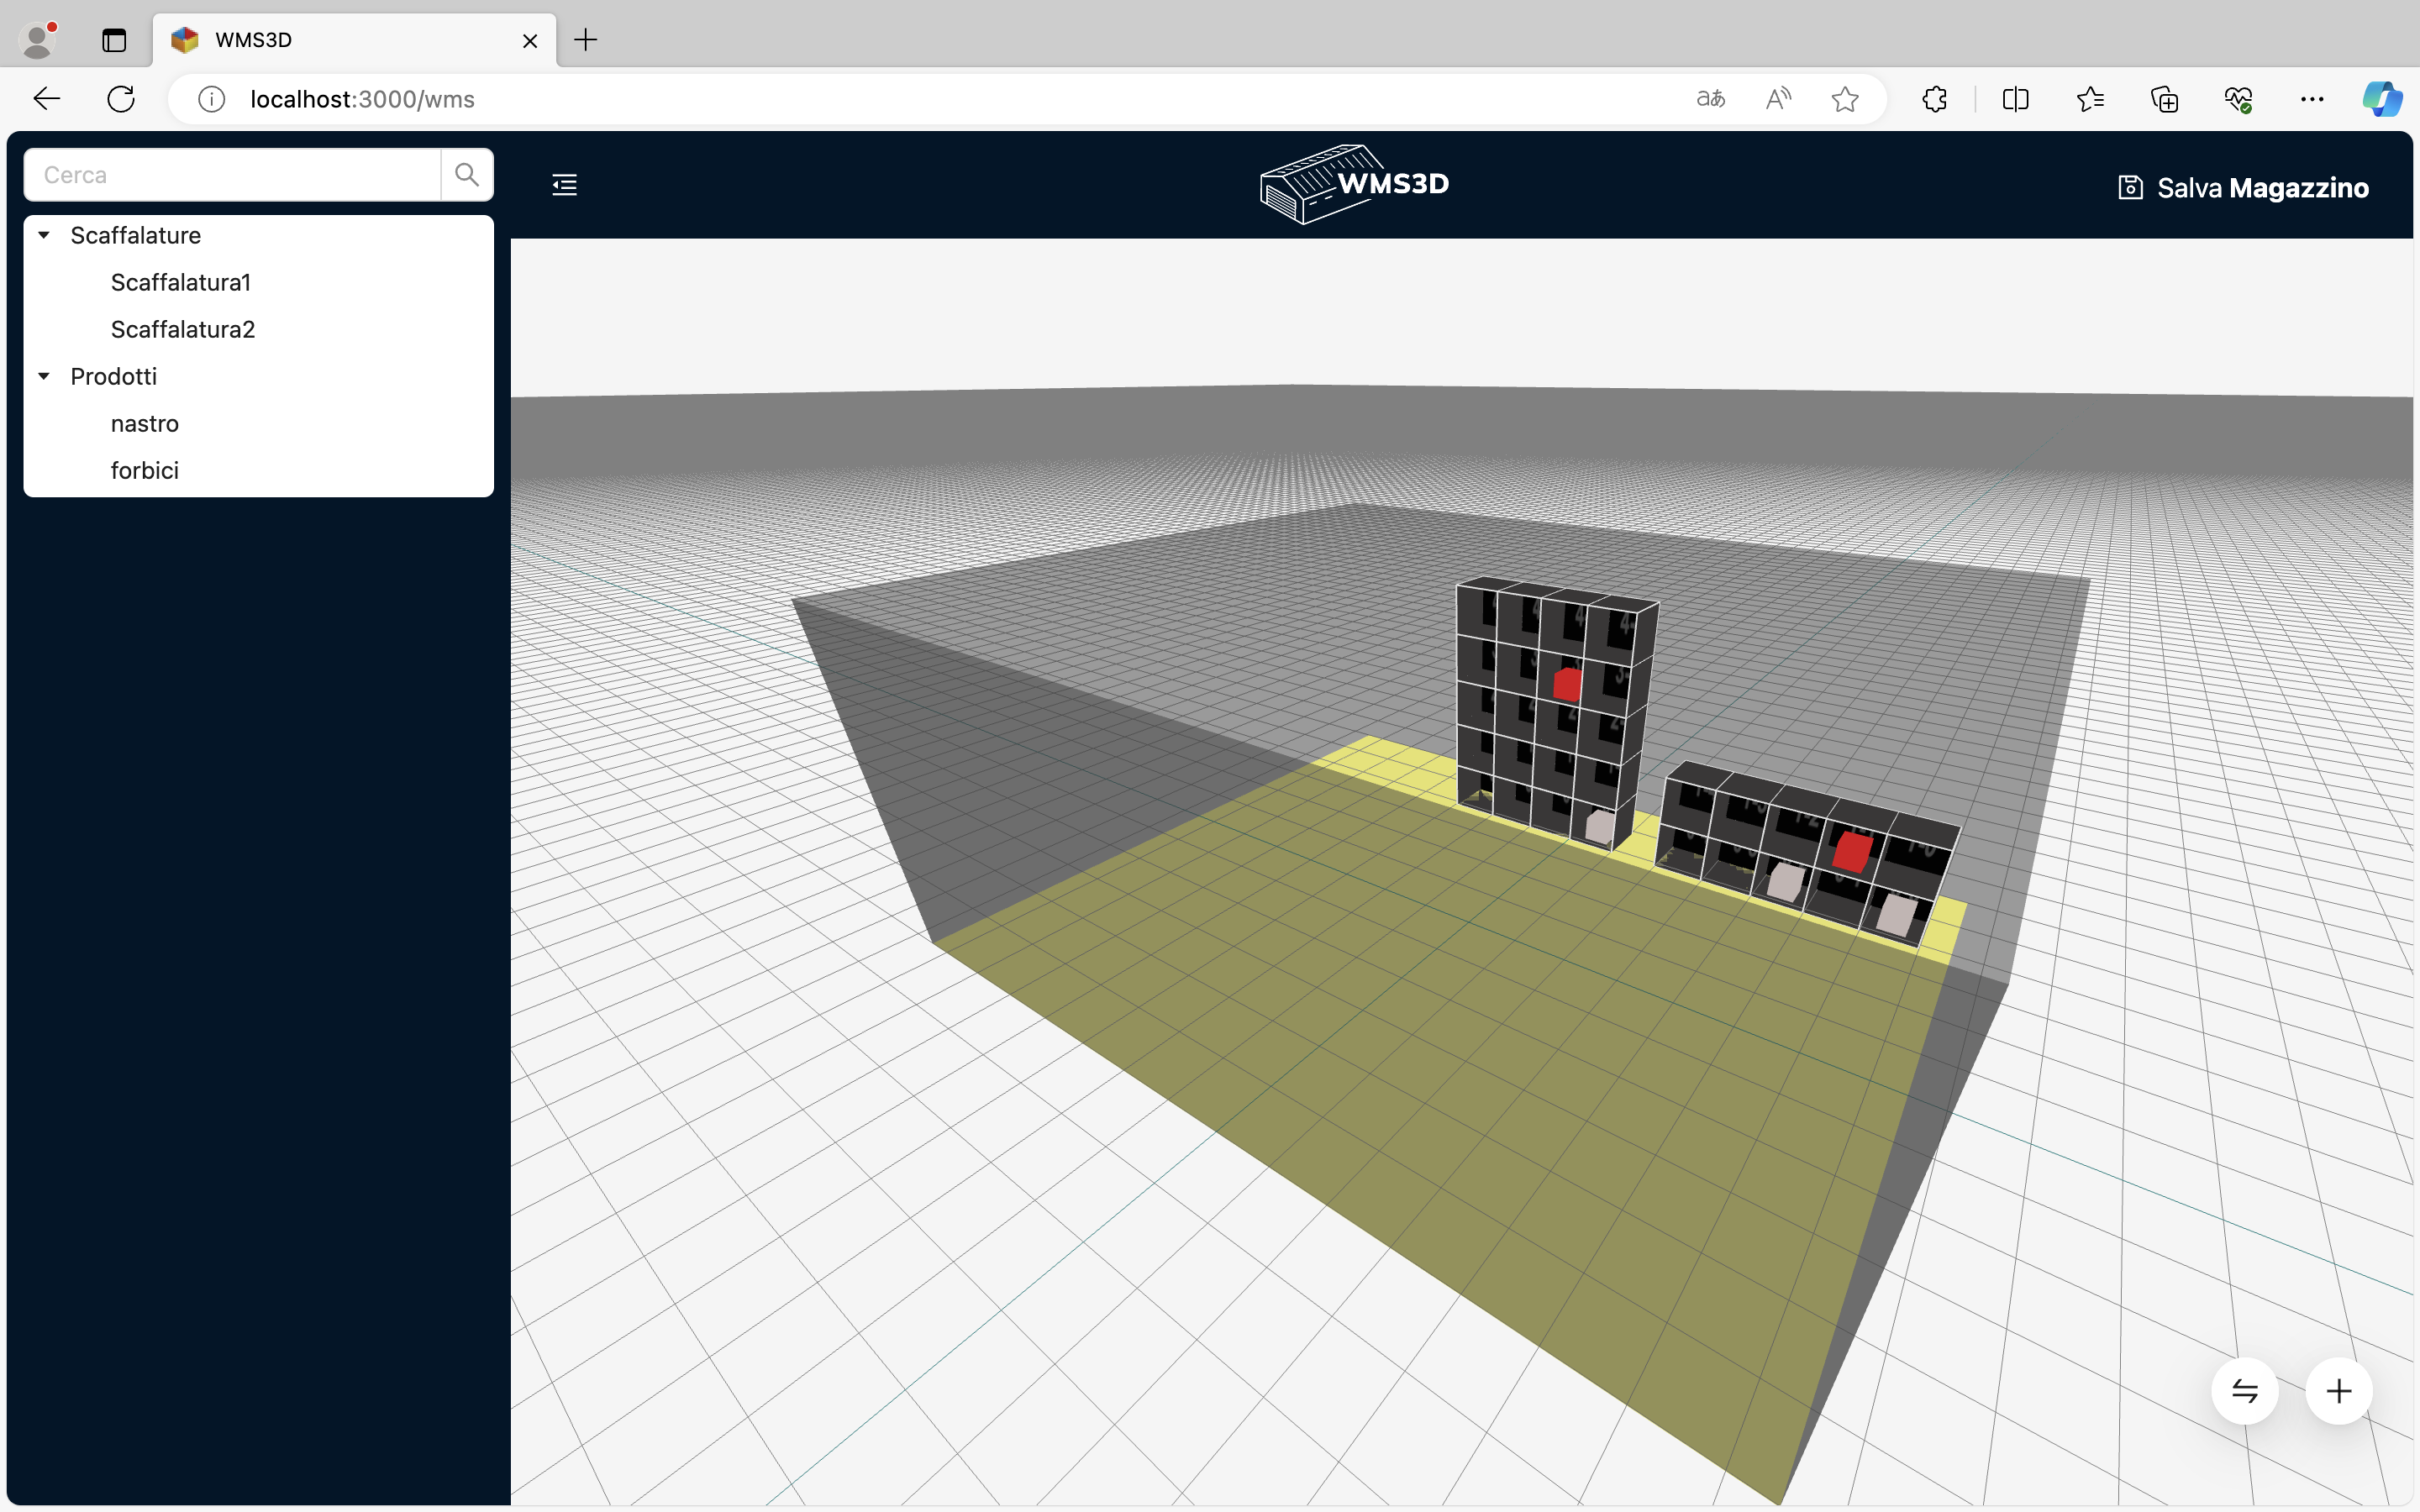
\includegraphics[width=0.8\textwidth]{images/microsoftedge.png}
    \caption{Test su Microsoft Edge}
\end{figure}
Versione: 124.0.2478.80 (Official build) (arm64)

\vspace{3cm}
\noindent
Come evidenziato nei precedenti paragrafi, la metrica MPD6-PPT è soddisfatta dato il corretto funzionamento dell'applicativo nei browser principali. 

\newpage
\section{Riferimenti esterni} \label{sec:riferimenti_esterni}
Per ulteriori chiarimenti sugli argomenti discussi nel documento, si possono consultare i seguenti link esterni:
\begin{itemize}
    \item \textbf{Piano di Progetto v2.0.0}:\\
    \url{https://github.com/Avant-Garde-Software-Engineering/WMS3D/blob/main/Documentazione/PB/Esterna/piano_di_progetto_v2.0.0.pdf}
    \item \textbf{Specifica Tecnica v1.0.0}:\\
    \url{https://github.com/Avant-Garde-Software-Engineering/WMS3D/blob/main/Documentazione/PB/Esterna/specifica_tecnica_v1.0.0.pdf}
    \item \textbf{Norme di Progetto v4.0.0}:\\
    \url{https://github.com/Avant-Garde-Software-Engineering/WMS3D/blob/main/Documentazione/PB/Interna/norme_di_progetto_v4.0.0.pdf}
    \item \textbf{Analisi dei Requisiti v5.0.0}:\\
    \url{https://github.com/Avant-Garde-Software-Engineering/WMS3D/blob/main/Documentazione/PB/Esterna/analisi_dei_requisiti_v5.0.0.pdf}
    \item \textbf{Glossario v1.0.0}:\\
    \url{https://github.com/Avant-Garde-Software-Engineering/WMS3D/blob/main/Documentazione/PB/Esterna/glossario_v1.0.0.pdf}
    \item Capitolato \textbf{Warehouse Management 3D}:\\
    \url{https://www.math.unipd.it/~tullio/IS-1/2023/Progetto/C5.pdf}
    \item \textbf{Regolamento} del progetto didattico:\\
    \url{https://www.math.unipd.it/~tullio/IS-1/2023/Dispense/PD2.pdf}
    \item Link alla \textbf{documentazione del gruppo}:\\
    \url{https://avant-garde-software-engineering.github.io/documentazione.html} \textcolor{gray}{\textit{(ultimo accesso 12-04-24)}}
    \item Standard \textbf{ISO/IEC 12207}, versione 1995:\\
    \url{https://www.math.unipd.it/~tullio/IS-1/2009/Approfondimenti/ISO_12207-1995.pdf}
    \item Metriche di progetto, metodo \textbf{Earned Value}:\\
    \url{https://it.wikipedia.org/wiki/Metriche_di_progetto} \textcolor{gray}{\textit{(ultimo accesso 12-04-24)}}
\end{itemize}